\documentclass[10pt]{article}
% Shared preamble for main.tex and appendix.tex
% RECOMB 2027 CFP: PDF, Letter, >= 10 pt, 1-inch margins, 10 pages incl. figures/tables/captions;
% extra title page allowed; bibliography not counted; appendix as separate PDF, no limit.
\usepackage[letterpaper,margin=1in]{geometry}
\usepackage[utf8]{inputenc}
\IfFileExists{lmodern.sty}{\usepackage[T1]{fontenc}\usepackage{lmodern}\usepackage{microtype}}{\usepackage[expansion=false]{microtype}}
\usepackage{amsmath,amssymb,amsthm,mathtools}
\usepackage{graphicx}
\usepackage{booktabs,longtable,multirow,array}
\usepackage{xcolor}
\usepackage{float}
\usepackage{caption}
\usepackage{subcaption}
\usepackage{enumitem}
\usepackage{tikz}
\usetikzlibrary{arrows.meta,positioning,shapes.geometric,fit,backgrounds}
\usepackage[ruled,vlined,linesnumbered]{algorithm2e}
\usepackage[numbers,sort&compress]{natbib}
\usepackage[colorlinks=true,linkcolor=blue!50!black,citecolor=green!40!black,urlcolor=blue!50!black]{hyperref}
\usepackage{url}

\captionsetup{font=small,labelfont=bf}
\setlist{nosep,leftmargin=*}

% ---- draft status colours (remove \pilot and \result before submission) ----
\definecolor{pilotc}{RGB}{214,110,0}
\newcommand{\pilot}[1]{\textcolor{pilotc}{#1}}            % pilot number, seeds 0-9: replace
\newcommand{\result}[1]{\textcolor{red}{[#1]}}             % pending confirmatory number
\newcommand{\todo}[1]{\textcolor{blue}{[TODO: #1]}}
\newcommand{\chk}[1]{\textcolor{magenta}{[CHECK: #1]}}   % needs advisor / verification

% ---- maths ----
\newtheorem{theorem}{Theorem}
\newtheorem{proposition}{Proposition}
\newtheorem{corollary}{Corollary}
\newtheorem{lemma}{Lemma}
\theoremstyle{definition}
\newtheorem{definition}{Definition}
\newtheorem{assumption}{Assumption}
\theoremstyle{remark}
\newtheorem{remark}{Remark}
\newcommand{\Prob}{\mathbb{P}}
\newcommand{\E}{\mathbb{E}}
\newcommand{\cov}{\mathrm{cov}}
\newcommand{\Cov}{\mathrm{Cov}}
\newcommand{\Beta}{\mathrm{Beta}}
\newcommand{\nreq}{n_{\mathrm{req}}}
\newcommand{\Dcal}{\mathcal{D}_{\mathrm{cal}}}
\newcommand{\bbbm}{BBB$-$}
\newcommand{\bbbp}{BBB$+$}
\newcommand{\SABM}{\textsc{SABM}}

% GENERATED by scripts/make_paper_numbers.py. Do not edit. Provenance: numbers_provenance.csv
\expandafter\def\csname v@marg.cls.min\endcsname{0.62}
\expandafter\def\csname v@marg.cls.max\endcsname{0.82}
\expandafter\def\csname v@mond.cls.min\endcsname{0.89}
\expandafter\def\csname v@mond.cls.max\endcsname{0.93}
\expandafter\def\csname v@mond.low.min\endcsname{0.79}
\expandafter\def\csname v@mond.low.max\endcsname{0.87}
\expandafter\def\csname v@mond.high.min\endcsname{0.94}
\expandafter\def\csname v@mond.high.max\endcsname{0.97}
\expandafter\def\csname v@mx.low.min\endcsname{0.88}
\expandafter\def\csname v@mx.low.max\endcsname{0.96}
\expandafter\def\csname v@mx.cls.min\endcsname{0.89}
\expandafter\def\csname v@mx.cls.max\endcsname{0.93}
\expandafter\def\csname v@size.cost.min\endcsname{0.009}
\expandafter\def\csname v@size.cost.max\endcsname{0.119}
\expandafter\def\csname v@mx.high.min\endcsname{0.85}
\expandafter\def\csname v@mx.high.max\endcsname{0.92}
\expandafter\def\csname v@mx.high.ndrop\endcsname{12}
\expandafter\def\csname v@mx.high.nbelow\endcsname{6}
\expandafter\def\csname v@mx.high.nciexcl\endcsname{0}
\expandafter\def\csname v@mx.low.nciexcl\endcsname{0}
\expandafter\def\csname v@rand.spread.min\endcsname{0.01}
\expandafter\def\csname v@rand.spread.max\endcsname{0.05}
\expandafter\def\csname v@mond.gap.min\endcsname{0.07}
\expandafter\def\csname v@mond.gap.max\endcsname{0.15}
\expandafter\def\csname v@n.lowcells.ciexcl\endcsname{10}
\expandafter\def\csname v@t.bbbp/random.rf.marginal.cov_minority\endcsname{0.65}
\expandafter\def\csname v@t.bbbp/random.rf.mondrian.cov_minority\endcsname{0.90}
\expandafter\def\csname v@t.bbbp/random.rf.mondrian.cov_min_bin0\endcsname{0.79}
\expandafter\def\csname v@t.bbbp/random.rf.mondrian.cov_min_bin2\endcsname{0.94}
\expandafter\def\csname v@t.bbbp/random.rf.mondrian.set_size\endcsname{1.17}
\expandafter\def\csname v@t.bbbp/random.rf.mondrian_x.cov_min_bin0\endcsname{0.93}
\expandafter\def\csname v@t.bbbp/random.rf.mondrian_x.set_size\endcsname{1.29}
\expandafter\def\csname v@t.bbbp/random.gin.marginal.cov_minority\endcsname{0.72}
\expandafter\def\csname v@t.bbbp/random.gin.mondrian.cov_minority\endcsname{0.91}
\expandafter\def\csname v@t.bbbp/random.gin.mondrian.cov_min_bin0\endcsname{0.81}
\expandafter\def\csname v@t.bbbp/random.gin.mondrian.cov_min_bin2\endcsname{0.95}
\expandafter\def\csname v@t.bbbp/random.gin.mondrian.set_size\endcsname{1.23}
\expandafter\def\csname v@t.bbbp/random.gin.mondrian_x.cov_min_bin0\endcsname{0.93}
\expandafter\def\csname v@t.bbbp/random.gin.mondrian_x.set_size\endcsname{1.30}
\expandafter\def\csname v@t.bbbp/random.chemprop.marginal.cov_minority\endcsname{0.75}
\expandafter\def\csname v@t.bbbp/random.chemprop.mondrian.cov_minority\endcsname{0.93}
\expandafter\def\csname v@t.bbbp/random.chemprop.mondrian.cov_min_bin0\endcsname{0.84}
\expandafter\def\csname v@t.bbbp/random.chemprop.mondrian.cov_min_bin2\endcsname{0.97}
\expandafter\def\csname v@t.bbbp/random.chemprop.mondrian.set_size\endcsname{1.23}
\expandafter\def\csname v@t.bbbp/random.chemprop.mondrian_x.cov_min_bin0\endcsname{0.96}
\expandafter\def\csname v@t.bbbp/random.chemprop.mondrian_x.set_size\endcsname{1.29}
\expandafter\def\csname v@t.bbbp/scaffold.rf.marginal.cov_minority\endcsname{0.62}
\expandafter\def\csname v@t.bbbp/scaffold.rf.mondrian.cov_minority\endcsname{0.89}
\expandafter\def\csname v@t.bbbp/scaffold.rf.mondrian.cov_min_bin0\endcsname{0.82}
\expandafter\def\csname v@t.bbbp/scaffold.rf.mondrian.cov_min_bin2\endcsname{0.96}
\expandafter\def\csname v@t.bbbp/scaffold.rf.mondrian.set_size\endcsname{1.28}
\expandafter\def\csname v@t.bbbp/scaffold.rf.mondrian_x.cov_min_bin0\endcsname{0.91}
\expandafter\def\csname v@t.bbbp/scaffold.rf.mondrian_x.set_size\endcsname{1.35}
\expandafter\def\csname v@t.bbbp/scaffold.gin.marginal.cov_minority\endcsname{0.69}
\expandafter\def\csname v@t.bbbp/scaffold.gin.mondrian.cov_minority\endcsname{0.91}
\expandafter\def\csname v@t.bbbp/scaffold.gin.mondrian.cov_min_bin0\endcsname{0.84}
\expandafter\def\csname v@t.bbbp/scaffold.gin.mondrian.cov_min_bin2\endcsname{0.96}
\expandafter\def\csname v@t.bbbp/scaffold.gin.mondrian.set_size\endcsname{1.34}
\expandafter\def\csname v@t.bbbp/scaffold.gin.mondrian_x.cov_min_bin0\endcsname{0.92}
\expandafter\def\csname v@t.bbbp/scaffold.gin.mondrian_x.set_size\endcsname{1.38}
\expandafter\def\csname v@t.bbbp/scaffold.chemprop.marginal.cov_minority\endcsname{0.71}
\expandafter\def\csname v@t.bbbp/scaffold.chemprop.mondrian.cov_minority\endcsname{0.91}
\expandafter\def\csname v@t.bbbp/scaffold.chemprop.mondrian.cov_min_bin0\endcsname{0.85}
\expandafter\def\csname v@t.bbbp/scaffold.chemprop.mondrian.cov_min_bin2\endcsname{0.97}
\expandafter\def\csname v@t.bbbp/scaffold.chemprop.mondrian.set_size\endcsname{1.32}
\expandafter\def\csname v@t.bbbp/scaffold.chemprop.mondrian_x.cov_min_bin0\endcsname{0.94}
\expandafter\def\csname v@t.bbbp/scaffold.chemprop.mondrian_x.set_size\endcsname{1.36}
\expandafter\def\csname v@t.b3db/random.rf.marginal.cov_minority\endcsname{0.79}
\expandafter\def\csname v@t.b3db/random.rf.mondrian.cov_minority\endcsname{0.91}
\expandafter\def\csname v@t.b3db/random.rf.mondrian.cov_min_bin0\endcsname{0.87}
\expandafter\def\csname v@t.b3db/random.rf.mondrian.cov_min_bin2\endcsname{0.94}
\expandafter\def\csname v@t.b3db/random.rf.mondrian.set_size\endcsname{1.26}
\expandafter\def\csname v@t.b3db/random.rf.mondrian_x.cov_min_bin0\endcsname{0.93}
\expandafter\def\csname v@t.b3db/random.rf.mondrian_x.set_size\endcsname{1.29}
\expandafter\def\csname v@t.b3db/random.gin.marginal.cov_minority\endcsname{0.82}
\expandafter\def\csname v@t.b3db/random.gin.mondrian.cov_minority\endcsname{0.91}
\expandafter\def\csname v@t.b3db/random.gin.mondrian.cov_min_bin0\endcsname{0.86}
\expandafter\def\csname v@t.b3db/random.gin.mondrian.cov_min_bin2\endcsname{0.96}
\expandafter\def\csname v@t.b3db/random.gin.mondrian.set_size\endcsname{1.33}
\expandafter\def\csname v@t.b3db/random.gin.mondrian_x.cov_min_bin0\endcsname{0.92}
\expandafter\def\csname v@t.b3db/random.gin.mondrian_x.set_size\endcsname{1.35}
\expandafter\def\csname v@t.b3db/random.chemprop.marginal.cov_minority\endcsname{0.81}
\expandafter\def\csname v@t.b3db/random.chemprop.mondrian.cov_minority\endcsname{0.91}
\expandafter\def\csname v@t.b3db/random.chemprop.mondrian.cov_min_bin0\endcsname{0.85}
\expandafter\def\csname v@t.b3db/random.chemprop.mondrian.cov_min_bin2\endcsname{0.96}
\expandafter\def\csname v@t.b3db/random.chemprop.mondrian.set_size\endcsname{1.32}
\expandafter\def\csname v@t.b3db/random.chemprop.mondrian_x.cov_min_bin0\endcsname{0.91}
\expandafter\def\csname v@t.b3db/random.chemprop.mondrian_x.set_size\endcsname{1.33}
\expandafter\def\csname v@t.b3db/scaffold.rf.marginal.cov_minority\endcsname{0.77}
\expandafter\def\csname v@t.b3db/scaffold.rf.mondrian.cov_minority\endcsname{0.89}
\expandafter\def\csname v@t.b3db/scaffold.rf.mondrian.cov_min_bin0\endcsname{0.84}
\expandafter\def\csname v@t.b3db/scaffold.rf.mondrian.cov_min_bin2\endcsname{0.94}
\expandafter\def\csname v@t.b3db/scaffold.rf.mondrian.set_size\endcsname{1.29}
\expandafter\def\csname v@t.b3db/scaffold.rf.mondrian_x.cov_min_bin0\endcsname{0.90}
\expandafter\def\csname v@t.b3db/scaffold.rf.mondrian_x.set_size\endcsname{1.30}
\expandafter\def\csname v@t.b3db/scaffold.gin.marginal.cov_minority\endcsname{0.81}
\expandafter\def\csname v@t.b3db/scaffold.gin.mondrian.cov_minority\endcsname{0.89}
\expandafter\def\csname v@t.b3db/scaffold.gin.mondrian.cov_min_bin0\endcsname{0.83}
\expandafter\def\csname v@t.b3db/scaffold.gin.mondrian.cov_min_bin2\endcsname{0.94}
\expandafter\def\csname v@t.b3db/scaffold.gin.mondrian.set_size\endcsname{1.33}
\expandafter\def\csname v@t.b3db/scaffold.gin.mondrian_x.cov_min_bin0\endcsname{0.88}
\expandafter\def\csname v@t.b3db/scaffold.gin.mondrian_x.set_size\endcsname{1.35}
\expandafter\def\csname v@t.b3db/scaffold.chemprop.marginal.cov_minority\endcsname{0.82}
\expandafter\def\csname v@t.b3db/scaffold.chemprop.mondrian.cov_minority\endcsname{0.89}
\expandafter\def\csname v@t.b3db/scaffold.chemprop.mondrian.cov_min_bin0\endcsname{0.85}
\expandafter\def\csname v@t.b3db/scaffold.chemprop.mondrian.cov_min_bin2\endcsname{0.95}
\expandafter\def\csname v@t.b3db/scaffold.chemprop.mondrian.set_size\endcsname{1.33}
\expandafter\def\csname v@t.b3db/scaffold.chemprop.mondrian_x.cov_min_bin0\endcsname{0.89}
\expandafter\def\csname v@t.b3db/scaffold.chemprop.mondrian_x.set_size\endcsname{1.35}
\expandafter\def\csname v@e.bbbptob3db/scaffold.rf.marginal.cov_minority\endcsname{0.38}
\expandafter\def\csname v@e.bbbptob3db/scaffold.rf.mondrian.cov_minority\endcsname{0.86}
\expandafter\def\csname v@e.bbbptob3db/scaffold.rf.mondrian.cov_min_bin0\endcsname{0.84}
\expandafter\def\csname v@e.bbbptob3db/scaffold.rf.mondrian_x.cov_min_bin0\endcsname{0.90}
\expandafter\def\csname v@e.bbbptob3db/scaffold.rf.mondrian.cov_majority\endcsname{0.77}
\expandafter\def\csname v@e.bbbptob3db/scaffold.rf.marginal.cov_majority\endcsname{0.98}
\expandafter\def\csname v@e.bbbptob3db/scaffold.rf.mondrian.set_size\endcsname{1.36}
\expandafter\def\csname v@e.bbbptob3db/scaffold.rf.mondrian_x.set_size\endcsname{1.45}
\expandafter\def\csname v@e.bbbptob3db/scaffold.rf.mondrian.cov_min_bin2\endcsname{0.91}
\expandafter\def\csname v@e.bbbptob3db/scaffold.gin.marginal.cov_minority\endcsname{0.50}
\expandafter\def\csname v@e.bbbptob3db/scaffold.gin.mondrian.cov_minority\endcsname{0.77}
\expandafter\def\csname v@e.bbbptob3db/scaffold.gin.mondrian.cov_min_bin0\endcsname{0.74}
\expandafter\def\csname v@e.bbbptob3db/scaffold.gin.mondrian_x.cov_min_bin0\endcsname{0.88}
\expandafter\def\csname v@e.bbbptob3db/scaffold.gin.mondrian.cov_majority\endcsname{0.81}
\expandafter\def\csname v@e.bbbptob3db/scaffold.gin.marginal.cov_majority\endcsname{0.92}
\expandafter\def\csname v@e.bbbptob3db/scaffold.gin.mondrian.set_size\endcsname{1.41}
\expandafter\def\csname v@e.bbbptob3db/scaffold.gin.mondrian_x.set_size\endcsname{1.51}
\expandafter\def\csname v@e.bbbptob3db/scaffold.gin.mondrian.cov_min_bin2\endcsname{0.87}
\expandafter\def\csname v@e.bbbptob3db/scaffold.chemprop.marginal.cov_minority\endcsname{0.51}
\expandafter\def\csname v@e.bbbptob3db/scaffold.chemprop.mondrian.cov_minority\endcsname{0.81}
\expandafter\def\csname v@e.bbbptob3db/scaffold.chemprop.mondrian.cov_min_bin0\endcsname{0.78}
\expandafter\def\csname v@e.bbbptob3db/scaffold.chemprop.mondrian_x.cov_min_bin0\endcsname{0.88}
\expandafter\def\csname v@e.bbbptob3db/scaffold.chemprop.mondrian.cov_majority\endcsname{0.79}
\expandafter\def\csname v@e.bbbptob3db/scaffold.chemprop.marginal.cov_majority\endcsname{0.95}
\expandafter\def\csname v@e.bbbptob3db/scaffold.chemprop.mondrian.set_size\endcsname{1.36}
\expandafter\def\csname v@e.bbbptob3db/scaffold.chemprop.mondrian_x.set_size\endcsname{1.46}
\expandafter\def\csname v@e.bbbptob3db/scaffold.chemprop.mondrian.cov_min_bin2\endcsname{0.90}
\expandafter\def\csname v@e.bbbp/cluster.rf.marginal.cov_minority\endcsname{0.54}
\expandafter\def\csname v@e.bbbp/cluster.rf.mondrian.cov_minority\endcsname{0.92}
\expandafter\def\csname v@e.bbbp/cluster.rf.mondrian.cov_min_bin0\endcsname{0.94}
\expandafter\def\csname v@e.bbbp/cluster.rf.mondrian_x.cov_min_bin0\endcsname{0.98}
\expandafter\def\csname v@e.bbbp/cluster.rf.mondrian.cov_majority\endcsname{0.79}
\expandafter\def\csname v@e.bbbp/cluster.rf.marginal.cov_majority\endcsname{0.99}
\expandafter\def\csname v@e.bbbp/cluster.rf.mondrian.set_size\endcsname{1.33}
\expandafter\def\csname v@e.bbbp/cluster.rf.mondrian_x.set_size\endcsname{1.46}
\expandafter\def\csname v@e.bbbp/cluster.rf.mondrian.cov_min_bin2\endcsname{0.75}
\expandafter\def\csname v@e.bbbp/cluster.gin.marginal.cov_minority\endcsname{0.69}
\expandafter\def\csname v@e.bbbp/cluster.gin.mondrian.cov_minority\endcsname{0.82}
\expandafter\def\csname v@e.bbbp/cluster.gin.mondrian.cov_min_bin0\endcsname{0.84}
\expandafter\def\csname v@e.bbbp/cluster.gin.mondrian_x.cov_min_bin0\endcsname{0.93}
\expandafter\def\csname v@e.bbbp/cluster.gin.mondrian.cov_majority\endcsname{0.83}
\expandafter\def\csname v@e.bbbp/cluster.gin.marginal.cov_majority\endcsname{0.93}
\expandafter\def\csname v@e.bbbp/cluster.gin.mondrian.set_size\endcsname{1.25}
\expandafter\def\csname v@e.bbbp/cluster.gin.mondrian_x.set_size\endcsname{1.38}
\expandafter\def\csname v@e.bbbp/cluster.gin.mondrian.cov_min_bin2\endcsname{0.72}
\expandafter\def\csname v@e.bbbp/cluster.chemprop.marginal.cov_minority\endcsname{0.65}
\expandafter\def\csname v@e.bbbp/cluster.chemprop.mondrian.cov_minority\endcsname{0.84}
\expandafter\def\csname v@e.bbbp/cluster.chemprop.mondrian.cov_min_bin0\endcsname{0.85}
\expandafter\def\csname v@e.bbbp/cluster.chemprop.mondrian_x.cov_min_bin0\endcsname{0.89}
\expandafter\def\csname v@e.bbbp/cluster.chemprop.mondrian.cov_majority\endcsname{0.84}
\expandafter\def\csname v@e.bbbp/cluster.chemprop.marginal.cov_majority\endcsname{0.93}
\expandafter\def\csname v@e.bbbp/cluster.chemprop.mondrian.set_size\endcsname{1.26}
\expandafter\def\csname v@e.bbbp/cluster.chemprop.mondrian_x.set_size\endcsname{1.36}
\expandafter\def\csname v@e.bbbp/cluster.chemprop.mondrian.cov_min_bin2\endcsname{0.73}
\expandafter\def\csname v@e.b3db/cluster.rf.marginal.cov_minority\endcsname{0.74}
\expandafter\def\csname v@e.b3db/cluster.rf.mondrian.cov_minority\endcsname{0.92}
\expandafter\def\csname v@e.b3db/cluster.rf.mondrian.cov_min_bin0\endcsname{0.92}
\expandafter\def\csname v@e.b3db/cluster.rf.mondrian_x.cov_min_bin0\endcsname{0.95}
\expandafter\def\csname v@e.b3db/cluster.rf.mondrian.cov_majority\endcsname{0.79}
\expandafter\def\csname v@e.b3db/cluster.rf.marginal.cov_majority\endcsname{0.98}
\expandafter\def\csname v@e.b3db/cluster.rf.mondrian.set_size\endcsname{1.45}
\expandafter\def\csname v@e.b3db/cluster.rf.mondrian_x.set_size\endcsname{1.52}
\expandafter\def\csname v@e.b3db/cluster.rf.mondrian.cov_min_bin2\endcsname{0.98}
\expandafter\def\csname v@e.b3db/cluster.gin.marginal.cov_minority\endcsname{0.74}
\expandafter\def\csname v@e.b3db/cluster.gin.mondrian.cov_minority\endcsname{0.83}
\expandafter\def\csname v@e.b3db/cluster.gin.mondrian.cov_min_bin0\endcsname{0.81}
\expandafter\def\csname v@e.b3db/cluster.gin.mondrian_x.cov_min_bin0\endcsname{0.86}
\expandafter\def\csname v@e.b3db/cluster.gin.mondrian.cov_majority\endcsname{0.87}
\expandafter\def\csname v@e.b3db/cluster.gin.marginal.cov_majority\endcsname{0.93}
\expandafter\def\csname v@e.b3db/cluster.gin.mondrian.set_size\endcsname{1.38}
\expandafter\def\csname v@e.b3db/cluster.gin.mondrian_x.set_size\endcsname{1.48}
\expandafter\def\csname v@e.b3db/cluster.gin.mondrian.cov_min_bin2\endcsname{0.86}
\expandafter\def\csname v@e.b3db/cluster.chemprop.marginal.cov_minority\endcsname{0.74}
\expandafter\def\csname v@e.b3db/cluster.chemprop.mondrian.cov_minority\endcsname{0.84}
\expandafter\def\csname v@e.b3db/cluster.chemprop.mondrian.cov_min_bin0\endcsname{0.83}
\expandafter\def\csname v@e.b3db/cluster.chemprop.mondrian_x.cov_min_bin0\endcsname{0.89}
\expandafter\def\csname v@e.b3db/cluster.chemprop.mondrian.cov_majority\endcsname{0.85}
\expandafter\def\csname v@e.b3db/cluster.chemprop.marginal.cov_majority\endcsname{0.92}
\expandafter\def\csname v@e.b3db/cluster.chemprop.mondrian.set_size\endcsname{1.36}
\expandafter\def\csname v@e.b3db/cluster.chemprop.mondrian_x.set_size\endcsname{1.48}
\expandafter\def\csname v@e.b3db/cluster.chemprop.mondrian.cov_min_bin2\endcsname{0.96}
\expandafter\def\csname v@data.bbbp.n\endcsname{1,924}
\expandafter\def\csname v@data.bbbp.minfrac\endcsname{23.5}
\expandafter\def\csname v@data.bbbp.nmin\endcsname{452}
\expandafter\def\csname v@data.b3db.n\endcsname{3,887}
\expandafter\def\csname v@data.b3db.minfrac\endcsname{36.5}
\expandafter\def\csname v@data.b3db.nmin\endcsname{1,417}
\expandafter\def\csname v@data.transfer.n\endcsname{2,119}
\expandafter\def\csname v@data.transfer.nmin\endcsname{1,070}
\expandafter\def\csname v@w.bbbp/random\endcsname{0.28}
\expandafter\def\csname v@floor.bbbp/random\endcsname{0.64}
\expandafter\def\csname v@w.bbbp/scaffold\endcsname{0.35}
\expandafter\def\csname v@floor.bbbp/scaffold\endcsname{0.71}
\expandafter\def\csname v@w.b3db/random\endcsname{0.35}
\expandafter\def\csname v@floor.b3db/random\endcsname{0.71}
\expandafter\def\csname v@w.b3db/scaffold\endcsname{0.37}
\expandafter\def\csname v@floor.b3db/scaffold\endcsname{0.73}
\expandafter\def\csname v@sec.aps.npos\endcsname{12}
\expandafter\def\csname v@sec.aps.ncell\endcsname{12}
\expandafter\def\csname v@sec.aps.gain.min\endcsname{0.03}
\expandafter\def\csname v@sec.aps.gain.max\endcsname{0.11}
\expandafter\def\csname v@sec.aps.mondlow.min\endcsname{0.82}
\expandafter\def\csname v@sec.aps.mondlow.max\endcsname{0.88}
\expandafter\def\csname v@sec.raps.npos\endcsname{12}
\expandafter\def\csname v@sec.raps.ncell\endcsname{12}
\expandafter\def\csname v@sec.raps.gain.min\endcsname{0.02}
\expandafter\def\csname v@sec.raps.gain.max\endcsname{0.13}
\expandafter\def\csname v@sec.raps.mondlow.min\endcsname{0.81}
\expandafter\def\csname v@sec.raps.mondlow.max\endcsname{0.87}
\expandafter\def\csname v@sec.a05.npos\endcsname{12}
\expandafter\def\csname v@sec.a05.ncell\endcsname{12}
\expandafter\def\csname v@sec.a05.gain.min\endcsname{0.02}
\expandafter\def\csname v@sec.a05.gain.max\endcsname{0.07}
\expandafter\def\csname v@sec.a05.mondlow.min\endcsname{0.91}
\expandafter\def\csname v@sec.a05.mondlow.max\endcsname{0.95}
\expandafter\def\csname v@sec.a20.npos\endcsname{12}
\expandafter\def\csname v@sec.a20.ncell\endcsname{12}
\expandafter\def\csname v@sec.a20.gain.min\endcsname{0.05}
\expandafter\def\csname v@sec.a20.gain.max\endcsname{0.24}
\expandafter\def\csname v@sec.a20.mondlow.min\endcsname{0.59}
\expandafter\def\csname v@sec.a20.mondlow.max\endcsname{0.75}
\expandafter\def\csname v@rob.mondrian_x_maccs.min\endcsname{0.85}
\expandafter\def\csname v@rob.mondrian_x_maccs.max\endcsname{0.92}
\expandafter\def\csname v@rob.mondrian_x_top5.min\endcsname{0.86}
\expandafter\def\csname v@rob.mondrian_x_top5.max\endcsname{0.93}
\expandafter\def\csname v@rob.mondrian_kmeans3.min\endcsname{0.83}
\expandafter\def\csname v@rob.mondrian_kmeans3.max\endcsname{0.88}
\expandafter\def\csname v@rob.mondrian_tpsa.min\endcsname{0.84}
\expandafter\def\csname v@rob.mondrian_tpsa.max\endcsname{0.89}
\expandafter\def\csname v@rob.mondrian_x_b2.min\endcsname{0.87}
\expandafter\def\csname v@rob.mondrian_x_b2.max\endcsname{0.95}
\expandafter\def\csname v@rob.mondrian_x_b5.min\endcsname{0.88}
\expandafter\def\csname v@rob.mondrian_x_b5.max\endcsname{0.97}
\expandafter\def\csname v@rob.mondrian_x_random.min\endcsname{0.83}
\expandafter\def\csname v@rob.mondrian_x_random.max\endcsname{0.89}
\expandafter\def\csname v@loss.rf.min\endcsname{0.00}
\expandafter\def\csname v@loss.rf.max\endcsname{0.01}
\expandafter\def\csname v@prem.rf.min\endcsname{-0.01}
\expandafter\def\csname v@prem.rf.max\endcsname{0.02}
\expandafter\def\csname v@loss.gin.min\endcsname{0.05}
\expandafter\def\csname v@loss.gin.max\endcsname{0.18}
\expandafter\def\csname v@prem.gin.min\endcsname{-0.15}
\expandafter\def\csname v@prem.gin.max\endcsname{-0.02}
\expandafter\def\csname v@loss.chemprop.min\endcsname{0.03}
\expandafter\def\csname v@loss.chemprop.max\endcsname{0.05}
\expandafter\def\csname v@prem.chemprop.min\endcsname{-0.03}
\expandafter\def\csname v@prem.chemprop.max\endcsname{0.00}
\expandafter\def\csname v@fam.size\endcsname{36}
\expandafter\def\csname v@gain.min\endcsname{0.045}
\expandafter\def\csname v@gain.max\endcsname{0.137}
\expandafter\def\csname v@gain.npos\endcsname{12}
\expandafter\def\csname v@gain.nsig\endcsname{9}
\expandafter\def\csname v@gain.bbbpscaf.holm\endcsname{0.077}
\expandafter\def\csname v@gain.bbbpscaf.min\endcsname{0.082}
\expandafter\def\csname v@gain.bbbpscaf.max\endcsname{0.091}
\expandafter\def\csname v@gain.sigmaxholm\endcsname{0.012}
\expandafter\def\csname v@gain.dz.min\endcsname{0.66}
\expandafter\def\csname v@gain.dz.max\endcsname{2.06}
\expandafter\def\csname v@sabmfixed.maxabs\endcsname{0.0000}
\expandafter\def\csname v@sabmfixed.nsig\endcsname{0}
\expandafter\def\csname v@boot.molecule.nsig\endcsname{12}
\expandafter\def\csname v@boot.molecule.maxholm\endcsname{0.0036}
\expandafter\def\csname v@boot.molecule.cilo.min\endcsname{0.035}
\expandafter\def\csname v@boot.molecule.cilo.max\endcsname{0.096}
\expandafter\def\csname v@boot.scaffold.nsig\endcsname{12}
\expandafter\def\csname v@boot.scaffold.maxholm\endcsname{0.0036}
\expandafter\def\csname v@boot.scaffold.cilo.min\endcsname{0.033}
\expandafter\def\csname v@boot.scaffold.cilo.max\endcsname{0.090}
\expandafter\def\csname v@boot.B\endcsname{20000}
\expandafter\def\csname v@boot.nmol.min\endcsname{158}
\expandafter\def\csname v@boot.nmol.max\endcsname{674}
\expandafter\def\csname v@cg.all.fixed_b2.t0.min\endcsname{0.87}
\expandafter\def\csname v@cg.all.fixed_b2.t0.max\endcsname{0.95}
\expandafter\def\csname v@cg.all.fixed_b2.size.min\endcsname{1.24}
\expandafter\def\csname v@cg.all.fixed_b2.size.max\endcsname{1.35}
\expandafter\def\csname v@cg.all.fixed_b2.single.min\endcsname{0.65}
\expandafter\def\csname v@cg.all.fixed_b2.single.max\endcsname{0.74}
\expandafter\def\csname v@cg.all.fixed_b3.t0.min\endcsname{0.88}
\expandafter\def\csname v@cg.all.fixed_b3.t0.max\endcsname{0.96}
\expandafter\def\csname v@cg.all.fixed_b3.size.min\endcsname{1.29}
\expandafter\def\csname v@cg.all.fixed_b3.size.max\endcsname{1.38}
\expandafter\def\csname v@cg.all.fixed_b3.single.min\endcsname{0.61}
\expandafter\def\csname v@cg.all.fixed_b3.single.max\endcsname{0.71}
\expandafter\def\csname v@cg.all.sabm_b3.t0.min\endcsname{0.88}
\expandafter\def\csname v@cg.all.sabm_b3.t0.max\endcsname{0.96}
\expandafter\def\csname v@cg.all.sabm_b3.size.min\endcsname{1.29}
\expandafter\def\csname v@cg.all.sabm_b3.size.max\endcsname{1.36}
\expandafter\def\csname v@cg.all.sabm_b3.single.min\endcsname{0.63}
\expandafter\def\csname v@cg.all.sabm_b3.single.max\endcsname{0.71}
\expandafter\def\csname v@cg.all.mondrian.t0.min\endcsname{0.79}
\expandafter\def\csname v@cg.all.mondrian.t0.max\endcsname{0.87}
\expandafter\def\csname v@cg.all.mondrian.size.min\endcsname{1.17}
\expandafter\def\csname v@cg.all.mondrian.size.max\endcsname{1.34}
\expandafter\def\csname v@cg.all.mondrian.single.min\endcsname{0.66}
\expandafter\def\csname v@cg.all.mondrian.single.max\endcsname{0.83}
\expandafter\def\csname v@cg.all.fixed_b5.t0.min\endcsname{0.88}
\expandafter\def\csname v@cg.all.fixed_b5.t0.max\endcsname{0.97}
\expandafter\def\csname v@cg.all.fixed_b5.size.min\endcsname{1.30}
\expandafter\def\csname v@cg.all.fixed_b5.size.max\endcsname{1.46}
\expandafter\def\csname v@cg.all.fixed_b5.single.min\endcsname{0.53}
\expandafter\def\csname v@cg.all.fixed_b5.single.max\endcsname{0.69}
\expandafter\def\csname v@cg.40.fixed_b2.t0.min\endcsname{0.90}
\expandafter\def\csname v@cg.40.fixed_b2.t0.max\endcsname{0.95}
\expandafter\def\csname v@cg.40.fixed_b2.size.min\endcsname{1.28}
\expandafter\def\csname v@cg.40.fixed_b2.size.max\endcsname{1.40}
\expandafter\def\csname v@cg.40.fixed_b2.single.min\endcsname{0.60}
\expandafter\def\csname v@cg.40.fixed_b2.single.max\endcsname{0.70}
\expandafter\def\csname v@cg.40.fixed_b3.t0.min\endcsname{0.91}
\expandafter\def\csname v@cg.40.fixed_b3.t0.max\endcsname{0.96}
\expandafter\def\csname v@cg.40.fixed_b3.size.min\endcsname{1.34}
\expandafter\def\csname v@cg.40.fixed_b3.size.max\endcsname{1.47}
\expandafter\def\csname v@cg.40.fixed_b3.single.min\endcsname{0.52}
\expandafter\def\csname v@cg.40.fixed_b3.single.max\endcsname{0.64}
\expandafter\def\csname v@cg.40.sabm_b3.t0.min\endcsname{0.90}
\expandafter\def\csname v@cg.40.sabm_b3.t0.max\endcsname{0.94}
\expandafter\def\csname v@cg.40.sabm_b3.size.min\endcsname{1.27}
\expandafter\def\csname v@cg.40.sabm_b3.size.max\endcsname{1.41}
\expandafter\def\csname v@cg.40.sabm_b3.single.min\endcsname{0.59}
\expandafter\def\csname v@cg.40.sabm_b3.single.max\endcsname{0.71}
\expandafter\def\csname v@cg.40.mondrian.t0.min\endcsname{0.78}
\expandafter\def\csname v@cg.40.mondrian.t0.max\endcsname{0.87}
\expandafter\def\csname v@cg.40.mondrian.size.min\endcsname{1.17}
\expandafter\def\csname v@cg.40.mondrian.size.max\endcsname{1.35}
\expandafter\def\csname v@cg.40.mondrian.single.min\endcsname{0.65}
\expandafter\def\csname v@cg.40.mondrian.single.max\endcsname{0.83}
\expandafter\def\csname v@cg.40.fixed_b5.t0.min\endcsname{0.94}
\expandafter\def\csname v@cg.40.fixed_b5.t0.max\endcsname{0.98}
\expandafter\def\csname v@cg.40.fixed_b5.size.min\endcsname{1.52}
\expandafter\def\csname v@cg.40.fixed_b5.size.max\endcsname{1.61}
\expandafter\def\csname v@cg.40.fixed_b5.single.min\endcsname{0.39}
\expandafter\def\csname v@cg.40.fixed_b5.single.max\endcsname{0.47}
\expandafter\def\csname v@cg.20.fixed_b2.t0.min\endcsname{0.92}
\expandafter\def\csname v@cg.20.fixed_b2.t0.max\endcsname{0.97}
\expandafter\def\csname v@cg.20.fixed_b2.size.min\endcsname{1.41}
\expandafter\def\csname v@cg.20.fixed_b2.size.max\endcsname{1.53}
\expandafter\def\csname v@cg.20.fixed_b2.single.min\endcsname{0.47}
\expandafter\def\csname v@cg.20.fixed_b2.single.max\endcsname{0.57}
\expandafter\def\csname v@cg.20.fixed_b3.t0.min\endcsname{0.95}
\expandafter\def\csname v@cg.20.fixed_b3.t0.max\endcsname{0.99}
\expandafter\def\csname v@cg.20.fixed_b3.size.min\endcsname{1.59}
\expandafter\def\csname v@cg.20.fixed_b3.size.max\endcsname{1.67}
\expandafter\def\csname v@cg.20.fixed_b3.single.min\endcsname{0.33}
\expandafter\def\csname v@cg.20.fixed_b3.single.max\endcsname{0.40}
\expandafter\def\csname v@cg.20.sabm_b3.t0.min\endcsname{0.80}
\expandafter\def\csname v@cg.20.sabm_b3.t0.max\endcsname{0.87}
\expandafter\def\csname v@cg.20.sabm_b3.size.min\endcsname{1.22}
\expandafter\def\csname v@cg.20.sabm_b3.size.max\endcsname{1.37}
\expandafter\def\csname v@cg.20.sabm_b3.single.min\endcsname{0.63}
\expandafter\def\csname v@cg.20.sabm_b3.single.max\endcsname{0.77}
\expandafter\def\csname v@cg.20.mondrian.t0.min\endcsname{0.80}
\expandafter\def\csname v@cg.20.mondrian.t0.max\endcsname{0.87}
\expandafter\def\csname v@cg.20.mondrian.size.min\endcsname{1.21}
\expandafter\def\csname v@cg.20.mondrian.size.max\endcsname{1.36}
\expandafter\def\csname v@cg.20.mondrian.single.min\endcsname{0.63}
\expandafter\def\csname v@cg.20.mondrian.single.max\endcsname{0.78}
\expandafter\def\csname v@cg.20.fixed_b5.t0.min\endcsname{0.99}
\expandafter\def\csname v@cg.20.fixed_b5.t0.max\endcsname{1.00}
\expandafter\def\csname v@cg.20.fixed_b5.size.min\endcsname{1.70}
\expandafter\def\csname v@cg.20.fixed_b5.size.max\endcsname{1.74}
\expandafter\def\csname v@cg.20.fixed_b5.single.min\endcsname{0.25}
\expandafter\def\csname v@cg.20.fixed_b5.single.max\endcsname{0.30}
\expandafter\def\csname v@cg.all.sabm_eq_b3\endcsname{12}
\expandafter\def\csname v@cg.ncells.all\endcsname{12}
\expandafter\def\csname v@cg.all.sabm3.size_eq\endcsname{8}
\expandafter\def\csname v@cg.all.sabm3.size_maxdiff\endcsname{0.026}
\expandafter\def\csname v@cg.all.fixed_b3.inf.max\endcsname{0.020}
\expandafter\def\csname v@cg.ncalmin.min\endcsname{65}
\expandafter\def\csname v@cg.ncalmin.max\endcsname{221}
\expandafter\def\csname v@fz.10.b2\endcsname{0.484}
\expandafter\def\csname v@fz.10.b3\endcsname{0.498}
\expandafter\def\csname v@fz.10.b5\endcsname{0.499}
\expandafter\def\csname v@fz.10.b8\endcsname{0.501}
\expandafter\def\csname v@fz.10.ncells\endcsname{12}
\expandafter\def\csname v@fz.20.b2\endcsname{0.160}
\expandafter\def\csname v@fz.20.b3\endcsname{0.379}
\expandafter\def\csname v@fz.20.b5\endcsname{0.481}
\expandafter\def\csname v@fz.20.b8\endcsname{0.498}
\expandafter\def\csname v@fz.20.ncells\endcsname{12}
\expandafter\def\csname v@fz.40.b2\endcsname{0.008}
\expandafter\def\csname v@fz.40.b3\endcsname{0.079}
\expandafter\def\csname v@fz.40.b5\endcsname{0.297}
\expandafter\def\csname v@fz.40.b8\endcsname{0.450}
\expandafter\def\csname v@fz.40.ncells\endcsname{12}
\expandafter\def\csname v@fz.80.b2\endcsname{0.000}
\expandafter\def\csname v@fz.80.b3\endcsname{0.000}
\expandafter\def\csname v@fz.80.b5\endcsname{0.034}
\expandafter\def\csname v@fz.80.b8\endcsname{0.190}
\expandafter\def\csname v@fz.80.ncells\endcsname{6}
\expandafter\def\csname v@fz.160.b2\endcsname{0.000}
\expandafter\def\csname v@fz.160.b3\endcsname{0.000}
\expandafter\def\csname v@fz.160.b5\endcsname{0.000}
\expandafter\def\csname v@fz.160.b8\endcsname{0.012}
\expandafter\def\csname v@fz.160.ncells\endcsname{6}
\expandafter\def\csname v@fz.all.b2\endcsname{0.000}
\expandafter\def\csname v@fz.all.b3\endcsname{0.006}
\expandafter\def\csname v@fz.all.b5\endcsname{0.065}
\expandafter\def\csname v@fz.all.b8\endcsname{0.154}
\expandafter\def\csname v@fz.all.ncells\endcsname{12}
\expandafter\def\csname v@cgm.40.fixed_b2.singleton_rate\endcsname{0.640}
\expandafter\def\csname v@cgm.40.fixed_b2.set_size\endcsname{1.354}
\expandafter\def\csname v@cgm.40.fixed_b2.cov_min_t0\endcsname{0.924}
\expandafter\def\csname v@cgm.40.sabm_b8.singleton_rate\endcsname{0.597}
\expandafter\def\csname v@cgm.40.sabm_b8.set_size\endcsname{1.396}
\expandafter\def\csname v@cgm.40.sabm_b8.cov_min_t0\endcsname{0.922}
\expandafter\def\csname v@cgm.40.fixed_b8.singleton_rate\endcsname{0.293}
\expandafter\def\csname v@cgm.40.fixed_b8.set_size\endcsname{1.703}
\expandafter\def\csname v@cgm.40.fixed_b8.cov_min_t0\endcsname{0.987}
\expandafter\def\csname v@cgm.40.mondrian.singleton_rate\endcsname{0.711}
\expandafter\def\csname v@cgm.40.mondrian.set_size\endcsname{1.289}
\expandafter\def\csname v@cgm.40.mondrian.cov_min_t0\endcsname{0.832}
\expandafter\def\csname v@cgm.all.fixed_b2.singleton_rate\endcsname{0.688}
\expandafter\def\csname v@cgm.all.fixed_b2.set_size\endcsname{1.308}
\expandafter\def\csname v@cgm.all.fixed_b2.cov_min_t0\endcsname{0.908}
\expandafter\def\csname v@cgm.all.sabm_b8.singleton_rate\endcsname{0.616}
\expandafter\def\csname v@cgm.all.sabm_b8.set_size\endcsname{1.374}
\expandafter\def\csname v@cgm.all.sabm_b8.cov_min_t0\endcsname{0.923}
\expandafter\def\csname v@cgm.all.fixed_b8.singleton_rate\endcsname{0.520}
\expandafter\def\csname v@cgm.all.fixed_b8.set_size\endcsname{1.471}
\expandafter\def\csname v@cgm.all.fixed_b8.cov_min_t0\endcsname{0.940}
\expandafter\def\csname v@cgm.all.mondrian.singleton_rate\endcsname{0.715}
\expandafter\def\csname v@cgm.all.mondrian.set_size\endcsname{1.285}
\expandafter\def\csname v@cgm.all.mondrian.cov_min_t0\endcsname{0.837}
\expandafter\def\csname v@cgm.20.fixed_b2.singleton_rate\endcsname{0.526}
\expandafter\def\csname v@cgm.20.fixed_b2.set_size\endcsname{1.466}
\expandafter\def\csname v@cgm.20.fixed_b2.cov_min_t0\endcsname{0.944}
\expandafter\def\csname v@cgm.20.sabm_b8.singleton_rate\endcsname{0.662}
\expandafter\def\csname v@cgm.20.sabm_b8.set_size\endcsname{1.336}
\expandafter\def\csname v@cgm.20.sabm_b8.cov_min_t0\endcsname{0.839}
\expandafter\def\csname v@cgm.20.fixed_b8.singleton_rate\endcsname{0.245}
\expandafter\def\csname v@cgm.20.fixed_b8.set_size\endcsname{1.754}
\expandafter\def\csname v@cgm.20.fixed_b8.cov_min_t0\endcsname{0.999}
\expandafter\def\csname v@cgm.20.mondrian.singleton_rate\endcsname{0.688}
\expandafter\def\csname v@cgm.20.mondrian.set_size\endcsname{1.311}
\expandafter\def\csname v@cgm.20.mondrian.cov_min_t0\endcsname{0.839}
\expandafter\def\csname v@pf.b3db/random.n_cross_arch\endcsname{10}
\expandafter\def\csname v@pf.b3db/random.n_eligible\endcsname{1149}
\expandafter\def\csname v@pf.b3db/random.n_majority_all3\endcsname{42}
\expandafter\def\csname v@pf.b3db/random.null\endcsname{0.09}
\expandafter\def\csname v@pf.b3db/random.p\endcsname{0.000}
\expandafter\def\csname v@pf.b3db/random.rf\endcsname{53}
\expandafter\def\csname v@pf.b3db/random.gin\endcsname{47}
\expandafter\def\csname v@pf.b3db/random.chemprop\endcsname{41}
\expandafter\def\csname v@pf.b3db/scaffold.n_cross_arch\endcsname{14}
\expandafter\def\csname v@pf.b3db/scaffold.n_eligible\endcsname{1199}
\expandafter\def\csname v@pf.b3db/scaffold.n_majority_all3\endcsname{55}
\expandafter\def\csname v@pf.b3db/scaffold.null\endcsname{0.21}
\expandafter\def\csname v@pf.b3db/scaffold.p\endcsname{0.000}
\expandafter\def\csname v@pf.b3db/scaffold.rf\endcsname{60}
\expandafter\def\csname v@pf.b3db/scaffold.gin\endcsname{66}
\expandafter\def\csname v@pf.b3db/scaffold.chemprop\endcsname{46}
\expandafter\def\csname v@pf.bbbp/random.n_cross_arch\endcsname{2}
\expandafter\def\csname v@pf.bbbp/random.n_eligible\endcsname{368}
\expandafter\def\csname v@pf.bbbp/random.n_majority_all3\endcsname{14}
\expandafter\def\csname v@pf.bbbp/random.null\endcsname{0.02}
\expandafter\def\csname v@pf.bbbp/random.p\endcsname{0.001}
\expandafter\def\csname v@pf.bbbp/random.rf\endcsname{19}
\expandafter\def\csname v@pf.bbbp/random.gin\endcsname{13}
\expandafter\def\csname v@pf.bbbp/random.chemprop\endcsname{9}
\expandafter\def\csname v@pf.bbbp/scaffold.n_cross_arch\endcsname{1}
\expandafter\def\csname v@pf.bbbp/scaffold.n_eligible\endcsname{386}
\expandafter\def\csname v@pf.bbbp/scaffold.n_majority_all3\endcsname{12}
\expandafter\def\csname v@pf.bbbp/scaffold.null\endcsname{0.02}
\expandafter\def\csname v@pf.bbbp/scaffold.p\endcsname{0.020}
\expandafter\def\csname v@pf.bbbp/scaffold.rf\endcsname{26}
\expandafter\def\csname v@pf.bbbp/scaffold.gin\endcsname{7}
\expandafter\def\csname v@pf.bbbp/scaffold.chemprop\endcsname{5}
\expandafter\def\csname v@pf.bbbptob3db/scaffold.n_cross_arch\endcsname{0}
\expandafter\def\csname v@pf.bbbptob3db/scaffold.n_eligible\endcsname{1070}
\expandafter\def\csname v@pf.bbbptob3db/scaffold.n_majority_all3\endcsname{46}
\expandafter\def\csname v@pf.bbbptob3db/scaffold.null\endcsname{0.00}
\expandafter\def\csname v@pf.bbbptob3db/scaffold.p\endcsname{1.000}
\expandafter\def\csname v@pf.bbbptob3db/scaffold.rf\endcsname{16}
\expandafter\def\csname v@pf.bbbptob3db/scaffold.gin\endcsname{16}
\expandafter\def\csname v@pf.bbbptob3db/scaffold.chemprop\endcsname{21}
\expandafter\def\csname v@pfx.b3db/random.n_cross_arch\endcsname{9}
\expandafter\def\csname v@pfx.b3db/random.null\endcsname{0.09}
\expandafter\def\csname v@pfx.b3db/scaffold.n_cross_arch\endcsname{12}
\expandafter\def\csname v@pfx.b3db/scaffold.null\endcsname{0.20}
\expandafter\def\csname v@pfx.bbbp/random.n_cross_arch\endcsname{2}
\expandafter\def\csname v@pfx.bbbp/random.null\endcsname{0.02}
\expandafter\def\csname v@pfx.bbbp/scaffold.n_cross_arch\endcsname{1}
\expandafter\def\csname v@pfx.bbbp/scaffold.null\endcsname{0.02}
\expandafter\def\csname v@pfx.bbbptob3db/scaffold.n_cross_arch\endcsname{0}
\expandafter\def\csname v@pfx.bbbptob3db/scaffold.null\endcsname{0.00}
\expandafter\def\csname v@pd.maj.b3db/random.TPSA.med\endcsname{36.8}
\expandafter\def\csname v@pd.maj.b3db/random.TPSA.rest\endcsname{94.8}
\expandafter\def\csname v@pd.maj.b3db/random.TPSA.holm\endcsname{0.000}
\expandafter\def\csname v@pd.maj.b3db/random.HBD.med\endcsname{1.00}
\expandafter\def\csname v@pd.maj.b3db/random.HBD.rest\endcsname{2.00}
\expandafter\def\csname v@pd.maj.b3db/random.HBD.holm\endcsname{0.000}
\expandafter\def\csname v@pd.maj.b3db/random.MW.med\endcsname{287.9}
\expandafter\def\csname v@pd.maj.b3db/random.MW.rest\endcsname{383.5}
\expandafter\def\csname v@pd.maj.b3db/random.MW.holm\endcsname{0.000}
\expandafter\def\csname v@pd.maj.b3db/random.cLogP.med\endcsname{2.65}
\expandafter\def\csname v@pd.maj.b3db/random.cLogP.rest\endcsname{2.11}
\expandafter\def\csname v@pd.maj.b3db/random.cLogP.holm\endcsname{0.286}
\expandafter\def\csname v@pd.maj.b3db/random.mean_sim_train.med\endcsname{0.37}
\expandafter\def\csname v@pd.maj.b3db/random.mean_sim_train.rest\endcsname{0.54}
\expandafter\def\csname v@pd.maj.b3db/scaffold.TPSA.med\endcsname{36.4}
\expandafter\def\csname v@pd.maj.b3db/scaffold.TPSA.rest\endcsname{95.9}
\expandafter\def\csname v@pd.maj.b3db/scaffold.TPSA.holm\endcsname{0.000}
\expandafter\def\csname v@pd.maj.b3db/scaffold.HBD.med\endcsname{1.00}
\expandafter\def\csname v@pd.maj.b3db/scaffold.HBD.rest\endcsname{2.00}
\expandafter\def\csname v@pd.maj.b3db/scaffold.HBD.holm\endcsname{0.000}
\expandafter\def\csname v@pd.maj.b3db/scaffold.MW.med\endcsname{288.4}
\expandafter\def\csname v@pd.maj.b3db/scaffold.MW.rest\endcsname{389.6}
\expandafter\def\csname v@pd.maj.b3db/scaffold.MW.holm\endcsname{0.000}
\expandafter\def\csname v@pd.maj.b3db/scaffold.cLogP.med\endcsname{2.92}
\expandafter\def\csname v@pd.maj.b3db/scaffold.cLogP.rest\endcsname{2.11}
\expandafter\def\csname v@pd.maj.b3db/scaffold.cLogP.holm\endcsname{0.083}
\expandafter\def\csname v@pd.maj.b3db/scaffold.mean_sim_train.med\endcsname{0.32}
\expandafter\def\csname v@pd.maj.b3db/scaffold.mean_sim_train.rest\endcsname{0.44}
\expandafter\def\csname v@pd.maj.bbbp/random.TPSA.med\endcsname{69.3}
\expandafter\def\csname v@pd.maj.bbbp/random.TPSA.rest\endcsname{112.7}
\expandafter\def\csname v@pd.maj.bbbp/random.TPSA.holm\endcsname{0.010}
\expandafter\def\csname v@pd.maj.bbbp/random.HBD.med\endcsname{2.00}
\expandafter\def\csname v@pd.maj.bbbp/random.HBD.rest\endcsname{3.00}
\expandafter\def\csname v@pd.maj.bbbp/random.HBD.holm\endcsname{0.027}
\expandafter\def\csname v@pd.maj.bbbp/random.MW.med\endcsname{313.1}
\expandafter\def\csname v@pd.maj.bbbp/random.MW.rest\endcsname{404.6}
\expandafter\def\csname v@pd.maj.bbbp/random.MW.holm\endcsname{0.286}
\expandafter\def\csname v@pd.maj.bbbp/random.cLogP.med\endcsname{3.04}
\expandafter\def\csname v@pd.maj.bbbp/random.cLogP.rest\endcsname{1.11}
\expandafter\def\csname v@pd.maj.bbbp/random.cLogP.holm\endcsname{0.027}
\expandafter\def\csname v@pd.maj.bbbp/random.mean_sim_train.med\endcsname{0.44}
\expandafter\def\csname v@pd.maj.bbbp/random.mean_sim_train.rest\endcsname{0.59}
\expandafter\def\csname v@pd.maj.bbbp/scaffold.TPSA.med\endcsname{63.9}
\expandafter\def\csname v@pd.maj.bbbp/scaffold.TPSA.rest\endcsname{111.9}
\expandafter\def\csname v@pd.maj.bbbp/scaffold.TPSA.holm\endcsname{0.010}
\expandafter\def\csname v@pd.maj.bbbp/scaffold.HBD.med\endcsname{2.00}
\expandafter\def\csname v@pd.maj.bbbp/scaffold.HBD.rest\endcsname{3.00}
\expandafter\def\csname v@pd.maj.bbbp/scaffold.HBD.holm\endcsname{0.009}
\expandafter\def\csname v@pd.maj.bbbp/scaffold.MW.med\endcsname{359.3}
\expandafter\def\csname v@pd.maj.bbbp/scaffold.MW.rest\endcsname{405.5}
\expandafter\def\csname v@pd.maj.bbbp/scaffold.MW.holm\endcsname{0.286}
\expandafter\def\csname v@pd.maj.bbbp/scaffold.cLogP.med\endcsname{2.87}
\expandafter\def\csname v@pd.maj.bbbp/scaffold.cLogP.rest\endcsname{1.33}
\expandafter\def\csname v@pd.maj.bbbp/scaffold.cLogP.holm\endcsname{0.092}
\expandafter\def\csname v@pd.maj.bbbp/scaffold.mean_sim_train.med\endcsname{0.30}
\expandafter\def\csname v@pd.maj.bbbp/scaffold.mean_sim_train.rest\endcsname{0.46}
\expandafter\def\csname v@pd.maj.bbbptob3db/scaffold.TPSA.med\endcsname{36.0}
\expandafter\def\csname v@pd.maj.bbbptob3db/scaffold.TPSA.rest\endcsname{89.1}
\expandafter\def\csname v@pd.maj.bbbptob3db/scaffold.TPSA.holm\endcsname{0.000}
\expandafter\def\csname v@pd.maj.bbbptob3db/scaffold.HBD.med\endcsname{1.00}
\expandafter\def\csname v@pd.maj.bbbptob3db/scaffold.HBD.rest\endcsname{2.00}
\expandafter\def\csname v@pd.maj.bbbptob3db/scaffold.HBD.holm\endcsname{0.000}
\expandafter\def\csname v@pd.maj.bbbptob3db/scaffold.MW.med\endcsname{287.9}
\expandafter\def\csname v@pd.maj.bbbptob3db/scaffold.MW.rest\endcsname{371.3}
\expandafter\def\csname v@pd.maj.bbbptob3db/scaffold.MW.holm\endcsname{0.000}
\expandafter\def\csname v@pd.maj.bbbptob3db/scaffold.cLogP.med\endcsname{2.80}
\expandafter\def\csname v@pd.maj.bbbptob3db/scaffold.cLogP.rest\endcsname{2.44}
\expandafter\def\csname v@pd.maj.bbbptob3db/scaffold.cLogP.holm\endcsname{0.286}
\expandafter\def\csname v@pd.maj.bbbptob3db/scaffold.mean_sim_train.med\endcsname{0.31}
\expandafter\def\csname v@pd.maj.bbbptob3db/scaffold.mean_sim_train.rest\endcsname{0.32}
\expandafter\def\csname v@pd.maj.tpsa.maxholm\endcsname{0.010}
\expandafter\def\csname v@pd.maj.tpsa.ntested\endcsname{5}
\expandafter\def\csname v@pd.maj.ntests\endcsname{20}
\expandafter\def\csname v@pd.str.b3db/random.TPSA.med\endcsname{34.1}
\expandafter\def\csname v@pd.str.b3db/random.TPSA.rest\endcsname{92.8}
\expandafter\def\csname v@pd.str.b3db/random.TPSA.holm\endcsname{0.000}
\expandafter\def\csname v@pd.str.b3db/random.HBD.med\endcsname{1.00}
\expandafter\def\csname v@pd.str.b3db/random.HBD.rest\endcsname{2.00}
\expandafter\def\csname v@pd.str.b3db/random.HBD.holm\endcsname{0.002}
\expandafter\def\csname v@pd.str.b3db/random.MW.med\endcsname{290.9}
\expandafter\def\csname v@pd.str.b3db/random.MW.rest\endcsname{380.5}
\expandafter\def\csname v@pd.str.b3db/random.MW.holm\endcsname{0.044}
\expandafter\def\csname v@pd.str.b3db/random.cLogP.med\endcsname{2.59}
\expandafter\def\csname v@pd.str.b3db/random.cLogP.rest\endcsname{2.12}
\expandafter\def\csname v@pd.str.b3db/random.cLogP.holm\endcsname{0.352}
\expandafter\def\csname v@pd.str.b3db/random.mean_sim_train.med\endcsname{0.41}
\expandafter\def\csname v@pd.str.b3db/random.mean_sim_train.rest\endcsname{0.53}
\expandafter\def\csname v@pd.str.b3db/scaffold.TPSA.med\endcsname{36.8}
\expandafter\def\csname v@pd.str.b3db/scaffold.TPSA.rest\endcsname{93.1}
\expandafter\def\csname v@pd.str.b3db/scaffold.TPSA.holm\endcsname{0.000}
\expandafter\def\csname v@pd.str.b3db/scaffold.HBD.med\endcsname{0.50}
\expandafter\def\csname v@pd.str.b3db/scaffold.HBD.rest\endcsname{2.00}
\expandafter\def\csname v@pd.str.b3db/scaffold.HBD.holm\endcsname{0.000}
\expandafter\def\csname v@pd.str.b3db/scaffold.MW.med\endcsname{269.6}
\expandafter\def\csname v@pd.str.b3db/scaffold.MW.rest\endcsname{384.6}
\expandafter\def\csname v@pd.str.b3db/scaffold.MW.holm\endcsname{0.001}
\expandafter\def\csname v@pd.str.b3db/scaffold.cLogP.med\endcsname{2.59}
\expandafter\def\csname v@pd.str.b3db/scaffold.cLogP.rest\endcsname{2.12}
\expandafter\def\csname v@pd.str.b3db/scaffold.cLogP.holm\endcsname{0.444}
\expandafter\def\csname v@pd.str.b3db/scaffold.mean_sim_train.med\endcsname{0.39}
\expandafter\def\csname v@pd.str.b3db/scaffold.mean_sim_train.rest\endcsname{0.44}
\expandafter\def\csname v@pd.str.bbbp/random.TPSA.med\endcsname{49.4}
\expandafter\def\csname v@pd.str.bbbp/random.TPSA.rest\endcsname{111.9}
\expandafter\def\csname v@pd.str.bbbp/random.HBD.med\endcsname{1.00}
\expandafter\def\csname v@pd.str.bbbp/random.HBD.rest\endcsname{3.00}
\expandafter\def\csname v@pd.str.bbbp/random.MW.med\endcsname{275.4}
\expandafter\def\csname v@pd.str.bbbp/random.MW.rest\endcsname{400.5}
\expandafter\def\csname v@pd.str.bbbp/random.cLogP.med\endcsname{2.57}
\expandafter\def\csname v@pd.str.bbbp/random.cLogP.rest\endcsname{1.22}
\expandafter\def\csname v@pd.str.bbbp/random.mean_sim_train.med\endcsname{0.54}
\expandafter\def\csname v@pd.str.bbbp/random.mean_sim_train.rest\endcsname{0.59}
\expandafter\def\csname v@pd.str.bbbp/scaffold.TPSA.med\endcsname{40.6}
\expandafter\def\csname v@pd.str.bbbp/scaffold.TPSA.rest\endcsname{110.4}
\expandafter\def\csname v@pd.str.bbbp/scaffold.HBD.med\endcsname{0.00}
\expandafter\def\csname v@pd.str.bbbp/scaffold.HBD.rest\endcsname{3.00}
\expandafter\def\csname v@pd.str.bbbp/scaffold.MW.med\endcsname{308.4}
\expandafter\def\csname v@pd.str.bbbp/scaffold.MW.rest\endcsname{403.8}
\expandafter\def\csname v@pd.str.bbbp/scaffold.cLogP.med\endcsname{3.79}
\expandafter\def\csname v@pd.str.bbbp/scaffold.cLogP.rest\endcsname{1.37}
\expandafter\def\csname v@pd.str.bbbp/scaffold.mean_sim_train.med\endcsname{0.35}
\expandafter\def\csname v@pd.str.bbbp/scaffold.mean_sim_train.rest\endcsname{0.46}
\expandafter\def\csname v@pd.str.bbbptob3db/scaffold.TPSA.med\endcsname{nan}
\expandafter\def\csname v@pd.str.bbbptob3db/scaffold.TPSA.rest\endcsname{87.3}
\expandafter\def\csname v@pd.str.bbbptob3db/scaffold.HBD.med\endcsname{nan}
\expandafter\def\csname v@pd.str.bbbptob3db/scaffold.HBD.rest\endcsname{2.00}
\expandafter\def\csname v@pd.str.bbbptob3db/scaffold.MW.med\endcsname{nan}
\expandafter\def\csname v@pd.str.bbbptob3db/scaffold.MW.rest\endcsname{366.4}
\expandafter\def\csname v@pd.str.bbbptob3db/scaffold.cLogP.med\endcsname{nan}
\expandafter\def\csname v@pd.str.bbbptob3db/scaffold.cLogP.rest\endcsname{2.47}
\expandafter\def\csname v@pd.str.bbbptob3db/scaffold.mean_sim_train.med\endcsname{nan}
\expandafter\def\csname v@pd.str.bbbptob3db/scaffold.mean_sim_train.rest\endcsname{0.32}
\expandafter\def\csname v@pd.str.tpsa.maxholm\endcsname{0.000}
\expandafter\def\csname v@pd.str.tpsa.ntested\endcsname{2}
\expandafter\def\csname v@pd.str.ntests\endcsname{8}
\expandafter\def\csname v@ev.b3db/random.p\endcsname{0.52}
\expandafter\def\csname v@ev.b3db/random.fp\endcsname{0.90}
\expandafter\def\csname v@ev.b3db/random.fr\endcsname{0.93}
\expandafter\def\csname v@ev.b3db/scaffold.p\endcsname{1.00}
\expandafter\def\csname v@ev.b3db/scaffold.fp\endcsname{0.93}
\expandafter\def\csname v@ev.b3db/scaffold.fr\endcsname{0.92}
\expandafter\def\csname v@adj.rf.unadj.min\endcsname{-3.07}
\expandafter\def\csname v@adj.rf.unadj.max\endcsname{-2.11}
\expandafter\def\csname v@adj.rf.sup.min\endcsname{-2.85}
\expandafter\def\csname v@adj.rf.sup.max\endcsname{-2.04}
\expandafter\def\csname v@adj.rf.perm.nsig\endcsname{4}
\expandafter\def\csname v@adj.gin.unadj.min\endcsname{-1.54}
\expandafter\def\csname v@adj.gin.unadj.max\endcsname{-0.89}
\expandafter\def\csname v@adj.gin.sup.min\endcsname{-1.36}
\expandafter\def\csname v@adj.gin.sup.max\endcsname{-0.46}
\expandafter\def\csname v@adj.gin.perm.nsig\endcsname{4}
\expandafter\def\csname v@adj.chemprop.unadj.min\endcsname{-2.01}
\expandafter\def\csname v@adj.chemprop.unadj.max\endcsname{-1.57}
\expandafter\def\csname v@adj.chemprop.sup.min\endcsname{-1.63}
\expandafter\def\csname v@adj.chemprop.sup.max\endcsname{-1.43}
\expandafter\def\csname v@adj.chemprop.perm.nsig\endcsname{4}
\expandafter\def\csname v@adj.nsup\endcsname{11}
\expandafter\def\csname v@adj.nfull\endcsname{9}
\expandafter\def\csname v@adj.ncells\endcsname{12}
\expandafter\def\csname v@su.ad_reject.minority_false_accept_rate.exch.min\endcsname{-0.16}
\expandafter\def\csname v@su.ad_reject.minority_false_accept_rate.exch.max\endcsname{-0.09}
\expandafter\def\csname v@su.ad_reject.minority_false_accept_rate.tr.min\endcsname{-0.24}
\expandafter\def\csname v@su.ad_reject.minority_false_accept_rate.tr.max\endcsname{-0.09}
\expandafter\def\csname v@su.ad_reject.minority_false_accept_rate.nneg\endcsname{15}
\expandafter\def\csname v@su.ad_reject.accepted_error.exch.min\endcsname{-0.04}
\expandafter\def\csname v@su.ad_reject.accepted_error.exch.max\endcsname{0.04}
\expandafter\def\csname v@su.ad_reject.accepted_error.tr.min\endcsname{-0.07}
\expandafter\def\csname v@su.ad_reject.accepted_error.tr.max\endcsname{0.00}
\expandafter\def\csname v@su.ad_reject.accepted_error.nneg\endcsname{8}
\expandafter\def\csname v@su.ad_reject.deferral_rate.exch.min\endcsname{0.00}
\expandafter\def\csname v@su.ad_reject.deferral_rate.exch.max\endcsname{0.00}
\expandafter\def\csname v@su.ad_reject.deferral_rate.tr.min\endcsname{0.00}
\expandafter\def\csname v@su.ad_reject.deferral_rate.tr.max\endcsname{0.00}
\expandafter\def\csname v@su.ad_reject.deferral_rate.nneg\endcsname{0}
\expandafter\def\csname v@su.ad_reject.low_support_accepted_error.exch.min\endcsname{-0.10}
\expandafter\def\csname v@su.ad_reject.low_support_accepted_error.exch.max\endcsname{0.11}
\expandafter\def\csname v@su.ad_reject.low_support_accepted_error.tr.min\endcsname{-0.11}
\expandafter\def\csname v@su.ad_reject.low_support_accepted_error.tr.max\endcsname{0.00}
\expandafter\def\csname v@su.ad_reject.low_support_accepted_error.nneg\endcsname{3}
\expandafter\def\csname v@su.conf_reject.minority_false_accept_rate.exch.min\endcsname{-0.10}
\expandafter\def\csname v@su.conf_reject.minority_false_accept_rate.exch.max\endcsname{-0.05}
\expandafter\def\csname v@su.conf_reject.minority_false_accept_rate.tr.min\endcsname{-0.25}
\expandafter\def\csname v@su.conf_reject.minority_false_accept_rate.tr.max\endcsname{-0.14}
\expandafter\def\csname v@su.conf_reject.minority_false_accept_rate.nneg\endcsname{15}
\expandafter\def\csname v@su.conf_reject.accepted_error.exch.min\endcsname{0.01}
\expandafter\def\csname v@su.conf_reject.accepted_error.exch.max\endcsname{0.10}
\expandafter\def\csname v@su.conf_reject.accepted_error.tr.min\endcsname{-0.06}
\expandafter\def\csname v@su.conf_reject.accepted_error.tr.max\endcsname{-0.01}
\expandafter\def\csname v@su.conf_reject.accepted_error.nneg\endcsname{3}
\expandafter\def\csname v@su.conf_reject.deferral_rate.exch.min\endcsname{0.00}
\expandafter\def\csname v@su.conf_reject.deferral_rate.exch.max\endcsname{0.00}
\expandafter\def\csname v@su.conf_reject.deferral_rate.tr.min\endcsname{0.00}
\expandafter\def\csname v@su.conf_reject.deferral_rate.tr.max\endcsname{0.00}
\expandafter\def\csname v@su.conf_reject.deferral_rate.nneg\endcsname{0}
\expandafter\def\csname v@su.conf_reject.low_support_accepted_error.exch.min\endcsname{-0.02}
\expandafter\def\csname v@su.conf_reject.low_support_accepted_error.exch.max\endcsname{0.14}
\expandafter\def\csname v@su.conf_reject.low_support_accepted_error.tr.min\endcsname{-0.09}
\expandafter\def\csname v@su.conf_reject.low_support_accepted_error.tr.max\endcsname{-0.03}
\expandafter\def\csname v@su.conf_reject.low_support_accepted_error.nneg\endcsname{4}
\expandafter\def\csname v@su.mondrian.minority_false_accept_rate.exch.min\endcsname{-0.03}
\expandafter\def\csname v@su.mondrian.minority_false_accept_rate.exch.max\endcsname{0.00}
\expandafter\def\csname v@su.mondrian.minority_false_accept_rate.tr.min\endcsname{-0.08}
\expandafter\def\csname v@su.mondrian.minority_false_accept_rate.tr.max\endcsname{-0.04}
\expandafter\def\csname v@su.mondrian.minority_false_accept_rate.nneg\endcsname{9}
\expandafter\def\csname v@su.mondrian.accepted_error.exch.min\endcsname{-0.01}
\expandafter\def\csname v@su.mondrian.accepted_error.exch.max\endcsname{0.00}
\expandafter\def\csname v@su.mondrian.accepted_error.tr.min\endcsname{-0.03}
\expandafter\def\csname v@su.mondrian.accepted_error.tr.max\endcsname{-0.02}
\expandafter\def\csname v@su.mondrian.accepted_error.nneg\endcsname{4}
\expandafter\def\csname v@su.mondrian.deferral_rate.exch.min\endcsname{0.01}
\expandafter\def\csname v@su.mondrian.deferral_rate.exch.max\endcsname{0.15}
\expandafter\def\csname v@su.mondrian.deferral_rate.tr.min\endcsname{0.11}
\expandafter\def\csname v@su.mondrian.deferral_rate.tr.max\endcsname{0.12}
\expandafter\def\csname v@su.mondrian.deferral_rate.nneg\endcsname{0}
\expandafter\def\csname v@su.mondrian.low_support_accepted_error.exch.min\endcsname{-0.07}
\expandafter\def\csname v@su.mondrian.low_support_accepted_error.exch.max\endcsname{0.03}
\expandafter\def\csname v@su.mondrian.low_support_accepted_error.tr.min\endcsname{-0.02}
\expandafter\def\csname v@su.mondrian.low_support_accepted_error.tr.max\endcsname{-0.02}
\expandafter\def\csname v@su.mondrian.low_support_accepted_error.nneg\endcsname{11}
\expandafter\def\csname v@su.mondrian_marginal.minority_false_accept_rate.exch.min\endcsname{-0.26}
\expandafter\def\csname v@su.mondrian_marginal.minority_false_accept_rate.exch.max\endcsname{-0.07}
\expandafter\def\csname v@su.mondrian_marginal.minority_false_accept_rate.tr.min\endcsname{-0.47}
\expandafter\def\csname v@su.mondrian_marginal.minority_false_accept_rate.tr.max\endcsname{-0.27}
\expandafter\def\csname v@su.mondrian_marginal.minority_false_accept_rate.nneg\endcsname{15}
\expandafter\def\csname v@su.mondrian_marginal.accepted_error.exch.min\endcsname{0.00}
\expandafter\def\csname v@su.mondrian_marginal.accepted_error.exch.max\endcsname{0.05}
\expandafter\def\csname v@su.mondrian_marginal.accepted_error.tr.min\endcsname{-0.10}
\expandafter\def\csname v@su.mondrian_marginal.accepted_error.tr.max\endcsname{-0.03}
\expandafter\def\csname v@su.mondrian_marginal.accepted_error.nneg\endcsname{3}
\expandafter\def\csname v@su.mondrian_marginal.deferral_rate.exch.min\endcsname{0.01}
\expandafter\def\csname v@su.mondrian_marginal.deferral_rate.exch.max\endcsname{0.19}
\expandafter\def\csname v@su.mondrian_marginal.deferral_rate.tr.min\endcsname{0.10}
\expandafter\def\csname v@su.mondrian_marginal.deferral_rate.tr.max\endcsname{0.17}
\expandafter\def\csname v@su.mondrian_marginal.deferral_rate.nneg\endcsname{0}
\expandafter\def\csname v@su.mondrian_marginal.low_support_accepted_error.exch.min\endcsname{-0.02}
\expandafter\def\csname v@su.mondrian_marginal.low_support_accepted_error.exch.max\endcsname{0.09}
\expandafter\def\csname v@su.mondrian_marginal.low_support_accepted_error.tr.min\endcsname{-0.11}
\expandafter\def\csname v@su.mondrian_marginal.low_support_accepted_error.tr.max\endcsname{-0.02}
\expandafter\def\csname v@su.mondrian_marginal.low_support_accepted_error.nneg\endcsname{3}
\expandafter\def\csname v@su.ad_reject_val.minority_false_accept_rate.exch.min\endcsname{-0.15}
\expandafter\def\csname v@su.ad_reject_val.minority_false_accept_rate.exch.max\endcsname{-0.09}
\expandafter\def\csname v@su.ad_reject_val.minority_false_accept_rate.tr.min\endcsname{-0.09}
\expandafter\def\csname v@su.ad_reject_val.minority_false_accept_rate.tr.max\endcsname{0.00}
\expandafter\def\csname v@su.ad_reject_val.minority_false_accept_rate.nneg\endcsname{14}
\expandafter\def\csname v@su.ad_reject_val.accepted_error.exch.min\endcsname{-0.04}
\expandafter\def\csname v@su.ad_reject_val.accepted_error.exch.max\endcsname{0.05}
\expandafter\def\csname v@su.ad_reject_val.accepted_error.tr.min\endcsname{-0.02}
\expandafter\def\csname v@su.ad_reject_val.accepted_error.tr.max\endcsname{0.03}
\expandafter\def\csname v@su.ad_reject_val.accepted_error.nneg\endcsname{6}
\expandafter\def\csname v@su.ad_reject_val.deferral_rate.exch.min\endcsname{-0.06}
\expandafter\def\csname v@su.ad_reject_val.deferral_rate.exch.max\endcsname{0.00}
\expandafter\def\csname v@su.ad_reject_val.deferral_rate.tr.min\endcsname{-0.17}
\expandafter\def\csname v@su.ad_reject_val.deferral_rate.tr.max\endcsname{-0.13}
\expandafter\def\csname v@su.ad_reject_val.deferral_rate.nneg\endcsname{5}
\expandafter\def\csname v@su.ad_reject_val.low_support_accepted_error.exch.min\endcsname{-0.06}
\expandafter\def\csname v@su.ad_reject_val.low_support_accepted_error.exch.max\endcsname{0.13}
\expandafter\def\csname v@su.ad_reject_val.low_support_accepted_error.tr.min\endcsname{-0.11}
\expandafter\def\csname v@su.ad_reject_val.low_support_accepted_error.tr.max\endcsname{0.01}
\expandafter\def\csname v@su.ad_reject_val.low_support_accepted_error.nneg\endcsname{2}
\expandafter\def\csname v@su.conf_reject_val.minority_false_accept_rate.exch.min\endcsname{-0.10}
\expandafter\def\csname v@su.conf_reject_val.minority_false_accept_rate.exch.max\endcsname{-0.05}
\expandafter\def\csname v@su.conf_reject_val.minority_false_accept_rate.tr.min\endcsname{-0.13}
\expandafter\def\csname v@su.conf_reject_val.minority_false_accept_rate.tr.max\endcsname{-0.10}
\expandafter\def\csname v@su.conf_reject_val.minority_false_accept_rate.nneg\endcsname{15}
\expandafter\def\csname v@su.conf_reject_val.accepted_error.exch.min\endcsname{0.01}
\expandafter\def\csname v@su.conf_reject_val.accepted_error.exch.max\endcsname{0.10}
\expandafter\def\csname v@su.conf_reject_val.accepted_error.tr.min\endcsname{-0.03}
\expandafter\def\csname v@su.conf_reject_val.accepted_error.tr.max\endcsname{-0.01}
\expandafter\def\csname v@su.conf_reject_val.accepted_error.nneg\endcsname{2}
\expandafter\def\csname v@su.conf_reject_val.deferral_rate.exch.min\endcsname{-0.05}
\expandafter\def\csname v@su.conf_reject_val.deferral_rate.exch.max\endcsname{0.01}
\expandafter\def\csname v@su.conf_reject_val.deferral_rate.tr.min\endcsname{-0.19}
\expandafter\def\csname v@su.conf_reject_val.deferral_rate.tr.max\endcsname{-0.03}
\expandafter\def\csname v@su.conf_reject_val.deferral_rate.nneg\endcsname{3}
\expandafter\def\csname v@su.conf_reject_val.low_support_accepted_error.exch.min\endcsname{-0.02}
\expandafter\def\csname v@su.conf_reject_val.low_support_accepted_error.exch.max\endcsname{0.15}
\expandafter\def\csname v@su.conf_reject_val.low_support_accepted_error.tr.min\endcsname{-0.06}
\expandafter\def\csname v@su.conf_reject_val.low_support_accepted_error.tr.max\endcsname{-0.03}
\expandafter\def\csname v@su.conf_reject_val.low_support_accepted_error.nneg\endcsname{4}
\expandafter\def\csname v@su.defer.exch.min\endcsname{0.29}
\expandafter\def\csname v@su.defer.exch.max\endcsname{0.39}
\expandafter\def\csname v@su.defer.tr.fixed_b3.min\endcsname{0.47}
\expandafter\def\csname v@su.defer.tr.fixed_b3.max\endcsname{0.53}
\expandafter\def\csname v@su.defer.tr.ad_reject_val.min\endcsname{0.64}
\expandafter\def\csname v@su.defer.tr.ad_reject_val.max\endcsname{0.66}
\expandafter\def\csname v@su.defer.tr.conf_reject_val.min\endcsname{0.56}
\expandafter\def\csname v@su.defer.tr.conf_reject_val.max\endcsname{0.66}
\expandafter\def\csname v@cb.marginal.low.min\endcsname{0.30}
\expandafter\def\csname v@cb.marginal.low.max\endcsname{0.76}
\expandafter\def\csname v@cb.marginal.high\endcsname{0.87}
\expandafter\def\csname v@cb.marginal.nfail\endcsname{12}
\expandafter\def\csname v@cb.marginal.size\endcsname{1.19}
\expandafter\def\csname v@cb.mondrian.low.min\endcsname{0.79}
\expandafter\def\csname v@cb.mondrian.low.max\endcsname{0.87}
\expandafter\def\csname v@cb.mondrian.high\endcsname{0.95}
\expandafter\def\csname v@cb.mondrian.nfail\endcsname{10}
\expandafter\def\csname v@cb.mondrian.size\endcsname{1.29}
\expandafter\def\csname v@cb.mondrian_x.low.min\endcsname{0.88}
\expandafter\def\csname v@cb.mondrian_x.low.max\endcsname{0.96}
\expandafter\def\csname v@cb.mondrian_x.high\endcsname{0.90}
\expandafter\def\csname v@cb.mondrian_x.nfail\endcsname{0}
\expandafter\def\csname v@cb.mondrian_x.size\endcsname{1.33}
\expandafter\def\csname v@cb.mondrian_pac.low.min\endcsname{0.86}
\expandafter\def\csname v@cb.mondrian_pac.low.max\endcsname{0.92}
\expandafter\def\csname v@cb.mondrian_pac.high\endcsname{0.97}
\expandafter\def\csname v@cb.mondrian_pac.nfail\endcsname{1}
\expandafter\def\csname v@cb.mondrian_pac.size\endcsname{1.40}
\expandafter\def\csname v@cb.mondrian_ssbc.low.min\endcsname{0.86}
\expandafter\def\csname v@cb.mondrian_ssbc.low.max\endcsname{0.92}
\expandafter\def\csname v@cb.mondrian_ssbc.high\endcsname{0.97}
\expandafter\def\csname v@cb.mondrian_ssbc.nfail\endcsname{1}
\expandafter\def\csname v@cb.mondrian_ssbc.size\endcsname{1.40}
\expandafter\def\csname v@cb.clustered_cells.low.min\endcsname{0.68}
\expandafter\def\csname v@cb.clustered_cells.low.max\endcsname{0.89}
\expandafter\def\csname v@cb.clustered_cells.high\endcsname{0.84}
\expandafter\def\csname v@cb.clustered_cells.nfail\endcsname{8}
\expandafter\def\csname v@cb.clustered_cells.size\endcsname{1.25}
\expandafter\def\csname v@cb.kandinsky_qr.low.min\endcsname{0.89}
\expandafter\def\csname v@cb.kandinsky_qr.low.max\endcsname{0.95}
\expandafter\def\csname v@cb.kandinsky_qr.high\endcsname{0.92}
\expandafter\def\csname v@cb.kandinsky_qr.nfail\endcsname{0}
\expandafter\def\csname v@cb.kandinsky_qr.size\endcsname{1.47}
\expandafter\def\csname v@cb.condqr_sim.low.min\endcsname{0.88}
\expandafter\def\csname v@cb.condqr_sim.low.max\endcsname{0.94}
\expandafter\def\csname v@cb.condqr_sim.high\endcsname{0.91}
\expandafter\def\csname v@cb.condqr_sim.nfail\endcsname{0}
\expandafter\def\csname v@cb.condqr_sim.size\endcsname{1.33}
\expandafter\def\csname v@cb.interp_q50.low.min\endcsname{0.52}
\expandafter\def\csname v@cb.interp_q50.low.max\endcsname{0.81}
\expandafter\def\csname v@cb.interp_q50.high\endcsname{0.91}
\expandafter\def\csname v@cb.interp_q50.nfail\endcsname{12}
\expandafter\def\csname v@cb.interp_q50.size\endcsname{1.22}
\expandafter\def\csname v@cb.interp_q90.low.min\endcsname{0.73}
\expandafter\def\csname v@cb.interp_q90.low.max\endcsname{0.85}
\expandafter\def\csname v@cb.interp_q90.high\endcsname{0.95}
\expandafter\def\csname v@cb.interp_q90.nfail\endcsname{12}
\expandafter\def\csname v@cb.interp_q90.size\endcsname{1.26}
\expandafter\def\csname v@cb.rc3p.low.min\endcsname{0.79}
\expandafter\def\csname v@cb.rc3p.low.max\endcsname{0.87}
\expandafter\def\csname v@cb.rc3p.high\endcsname{0.95}
\expandafter\def\csname v@cb.rc3p.nfail\endcsname{10}
\expandafter\def\csname v@cb.rc3p.size\endcsname{1.31}
\expandafter\def\csname v@cb.lcp_tanimoto.low.min\endcsname{0.86}
\expandafter\def\csname v@cb.lcp_tanimoto.low.max\endcsname{0.98}
\expandafter\def\csname v@cb.lcp_tanimoto.high\endcsname{0.97}
\expandafter\def\csname v@cb.lcp_tanimoto.nfail\endcsname{1}
\expandafter\def\csname v@cb.lcp_tanimoto.size\endcsname{1.47}
\expandafter\def\csname v@cb.lcp_knn.low.min\endcsname{0.80}
\expandafter\def\csname v@cb.lcp_knn.low.max\endcsname{0.89}
\expandafter\def\csname v@cb.lcp_knn.high\endcsname{0.95}
\expandafter\def\csname v@cb.lcp_knn.nfail\endcsname{8}
\expandafter\def\csname v@cb.lcp_knn.size\endcsname{1.33}
\expandafter\def\csname v@cb.rlcp_sim.low.min\endcsname{0.86}
\expandafter\def\csname v@cb.rlcp_sim.low.max\endcsname{0.94}
\expandafter\def\csname v@cb.rlcp_sim.high\endcsname{0.92}
\expandafter\def\csname v@cb.rlcp_sim.nfail\endcsname{1}
\expandafter\def\csname v@cb.rlcp_sim.size\endcsname{1.32}
\expandafter\def\csname v@cb.weighted_mondrian.low.min\endcsname{0.78}
\expandafter\def\csname v@cb.weighted_mondrian.low.max\endcsname{0.91}
\expandafter\def\csname v@cb.weighted_mondrian.high\endcsname{0.96}
\expandafter\def\csname v@cb.weighted_mondrian.nfail\endcsname{7}
\expandafter\def\csname v@cb.weighted_mondrian.size\endcsname{1.34}
\expandafter\def\csname v@cb.kmm_mondrian.low.min\endcsname{0.76}
\expandafter\def\csname v@cb.kmm_mondrian.low.max\endcsname{0.87}
\expandafter\def\csname v@cb.kmm_mondrian.high\endcsname{0.95}
\expandafter\def\csname v@cb.kmm_mondrian.nfail\endcsname{11}
\expandafter\def\csname v@cb.kmm_mondrian.size\endcsname{1.28}
\expandafter\def\csname v@cb.macro_cov.low.min\endcsname{0.62}
\expandafter\def\csname v@cb.macro_cov.low.max\endcsname{0.80}
\expandafter\def\csname v@cb.macro_cov.high\endcsname{0.92}
\expandafter\def\csname v@cb.macro_cov.nfail\endcsname{12}
\expandafter\def\csname v@cb.macro_cov.size\endcsname{1.31}
\expandafter\def\csname v@rs.gain.min\endcsname{0.036}
\expandafter\def\csname v@rs.gain.max\endcsname{0.100}
\expandafter\def\csname v@rs.npos\endcsname{12}
\expandafter\def\csname v@rs.nsig\endcsname{10}
\expandafter\def\csname v@rs.fam\endcsname{12}
\expandafter\def\csname v@rs.nonsig.maxholm\endcsname{0.099}
\expandafter\def\csname v@rs.nonsig.n\endcsname{2}
\expandafter\def\csname v@rs.randlow.min\endcsname{0.83}
\expandafter\def\csname v@rs.randlow.max\endcsname{0.89}
\expandafter\def\csname v@rs.cellsize.low.min\endcsname{0.008}
\expandafter\def\csname v@rs.cellsize.low.max\endcsname{0.045}
\expandafter\def\csname v@rs.cellsize.high.min\endcsname{-0.002}
\expandafter\def\csname v@rs.cellsize.high.max\endcsname{0.022}
\expandafter\def\csname v@rs.randhigh.nup\endcsname{11}
\expandafter\def\csname v@rs.randsize.min\endcsname{1.27}
\expandafter\def\csname v@rs.randsize.max\endcsname{1.41}
\expandafter\def\csname v@rs.cellsize.low.bbbp.min\endcsname{0.010}
\expandafter\def\csname v@rs.cellsize.low.bbbp.max\endcsname{0.045}
\expandafter\def\csname v@th.csb.bbbp.min\endcsname{0.043}
\expandafter\def\csname v@th.csb.bbbp.max\endcsname{0.044}
\expandafter\def\csname v@rs.cellsize.low.b3db.min\endcsname{0.008}
\expandafter\def\csname v@rs.cellsize.low.b3db.max\endcsname{0.016}
\expandafter\def\csname v@th.csb.b3db.min\endcsname{0.013}
\expandafter\def\csname v@th.csb.b3db.max\endcsname{0.014}
\expandafter\def\csname v@rs.mxsize.min\endcsname{1.29}
\expandafter\def\csname v@rs.mxsize.max\endcsname{1.38}
\expandafter\def\csname v@perf.auroc.min\endcsname{0.84}
\expandafter\def\csname v@perf.auroc.max\endcsname{0.91}
\expandafter\def\csname v@perf.tr.auroc.min\endcsname{0.65}
\expandafter\def\csname v@perf.tr.auroc.max\endcsname{0.72}
\expandafter\def\csname v@perf.auprc.min\endcsname{0.73}
\expandafter\def\csname v@perf.auprc.max\endcsname{0.82}
\expandafter\def\csname v@perf.tr.auprc.min\endcsname{0.68}
\expandafter\def\csname v@perf.tr.auprc.max\endcsname{0.73}
\expandafter\def\csname v@perf.balacc.min\endcsname{0.73}
\expandafter\def\csname v@perf.balacc.max\endcsname{0.81}
\expandafter\def\csname v@perf.tr.balacc.min\endcsname{0.58}
\expandafter\def\csname v@perf.tr.balacc.max\endcsname{0.60}
\expandafter\def\csname v@perf.minrecall.min\endcsname{0.49}
\expandafter\def\csname v@perf.minrecall.max\endcsname{0.69}
\expandafter\def\csname v@perf.tr.minrecall.min\endcsname{0.19}
\expandafter\def\csname v@perf.tr.minrecall.max\endcsname{0.35}
\expandafter\def\csname v@perf.prev.min\endcsname{0.24}
\expandafter\def\csname v@perf.prev.max\endcsname{0.37}
\expandafter\def\csname v@perf.tr.prev.min\endcsname{0.50}
\expandafter\def\csname v@perf.tr.prev.max\endcsname{0.50}
\expandafter\def\csname v@cr.mond_ad.minority_false_accept_rate.exch.min\endcsname{-0.004}
\expandafter\def\csname v@cr.mond_ad.minority_false_accept_rate.exch.max\endcsname{0.014}
\expandafter\def\csname v@cr.mond_ad.minority_false_accept_rate.tr.min\endcsname{-0.009}
\expandafter\def\csname v@cr.mond_ad.minority_false_accept_rate.tr.max\endcsname{-0.004}
\expandafter\def\csname v@cr.mond_ad.minority_false_accept_rate.nlow\endcsname{0}
\expandafter\def\csname v@cr.mond_ad.minority_false_accept_rate.nhigh\endcsname{0}
\expandafter\def\csname v@cr.mond_ad.accepted_error.exch.min\endcsname{0.000}
\expandafter\def\csname v@cr.mond_ad.accepted_error.exch.max\endcsname{0.014}
\expandafter\def\csname v@cr.mond_ad.accepted_error.tr.min\endcsname{-0.001}
\expandafter\def\csname v@cr.mond_ad.accepted_error.tr.max\endcsname{0.007}
\expandafter\def\csname v@cr.mond_ad.accepted_error.nlow\endcsname{0}
\expandafter\def\csname v@cr.mond_ad.accepted_error.nhigh\endcsname{5}
\expandafter\def\csname v@cr.mond_ad.deferral_rate.exch.min\endcsname{-0.015}
\expandafter\def\csname v@cr.mond_ad.deferral_rate.exch.max\endcsname{0.000}
\expandafter\def\csname v@cr.mond_ad.deferral_rate.tr.min\endcsname{-0.003}
\expandafter\def\csname v@cr.mond_ad.deferral_rate.tr.max\endcsname{0.000}
\expandafter\def\csname v@cr.mond_ad.deferral_rate.nlow\endcsname{8}
\expandafter\def\csname v@cr.mond_ad.deferral_rate.nhigh\endcsname{0}
\expandafter\def\csname v@cr.mond_conf.minority_false_accept_rate.exch.min\endcsname{-0.025}
\expandafter\def\csname v@cr.mond_conf.minority_false_accept_rate.exch.max\endcsname{-0.002}
\expandafter\def\csname v@cr.mond_conf.minority_false_accept_rate.tr.min\endcsname{-0.065}
\expandafter\def\csname v@cr.mond_conf.minority_false_accept_rate.tr.max\endcsname{-0.041}
\expandafter\def\csname v@cr.mond_conf.minority_false_accept_rate.nlow\endcsname{9}
\expandafter\def\csname v@cr.mond_conf.minority_false_accept_rate.nhigh\endcsname{0}
\expandafter\def\csname v@cr.mond_conf.accepted_error.exch.min\endcsname{0.005}
\expandafter\def\csname v@cr.mond_conf.accepted_error.exch.max\endcsname{0.042}
\expandafter\def\csname v@cr.mond_conf.accepted_error.tr.min\endcsname{-0.022}
\expandafter\def\csname v@cr.mond_conf.accepted_error.tr.max\endcsname{-0.009}
\expandafter\def\csname v@cr.mond_conf.accepted_error.nlow\endcsname{2}
\expandafter\def\csname v@cr.mond_conf.accepted_error.nhigh\endcsname{12}
\expandafter\def\csname v@cr.mond_conf.deferral_rate.exch.min\endcsname{-0.015}
\expandafter\def\csname v@cr.mond_conf.deferral_rate.exch.max\endcsname{0.000}
\expandafter\def\csname v@cr.mond_conf.deferral_rate.tr.min\endcsname{-0.003}
\expandafter\def\csname v@cr.mond_conf.deferral_rate.tr.max\endcsname{0.000}
\expandafter\def\csname v@cr.mond_conf.deferral_rate.nlow\endcsname{8}
\expandafter\def\csname v@cr.mond_conf.deferral_rate.nhigh\endcsname{0}
\expandafter\def\csname v@cr.mond_ad_val.minority_false_accept_rate.exch.min\endcsname{-0.002}
\expandafter\def\csname v@cr.mond_ad_val.minority_false_accept_rate.exch.max\endcsname{0.017}
\expandafter\def\csname v@cr.mond_ad_val.minority_false_accept_rate.tr.min\endcsname{0.003}
\expandafter\def\csname v@cr.mond_ad_val.minority_false_accept_rate.tr.max\endcsname{0.026}
\expandafter\def\csname v@cr.mond_ad_val.minority_false_accept_rate.nlow\endcsname{0}
\expandafter\def\csname v@cr.mond_ad_val.minority_false_accept_rate.nhigh\endcsname{2}
\expandafter\def\csname v@cr.mond_ad_val.accepted_error.exch.min\endcsname{0.001}
\expandafter\def\csname v@cr.mond_ad_val.accepted_error.exch.max\endcsname{0.022}
\expandafter\def\csname v@cr.mond_ad_val.accepted_error.tr.min\endcsname{0.010}
\expandafter\def\csname v@cr.mond_ad_val.accepted_error.tr.max\endcsname{0.030}
\expandafter\def\csname v@cr.mond_ad_val.accepted_error.nlow\endcsname{0}
\expandafter\def\csname v@cr.mond_ad_val.accepted_error.nhigh\endcsname{7}
\expandafter\def\csname v@cr.mond_ad_val.deferral_rate.exch.min\endcsname{-0.038}
\expandafter\def\csname v@cr.mond_ad_val.deferral_rate.exch.max\endcsname{0.007}
\expandafter\def\csname v@cr.mond_ad_val.deferral_rate.tr.min\endcsname{-0.117}
\expandafter\def\csname v@cr.mond_ad_val.deferral_rate.tr.max\endcsname{-0.025}
\expandafter\def\csname v@cr.mond_ad_val.deferral_rate.nlow\endcsname{5}
\expandafter\def\csname v@cr.mond_ad_val.deferral_rate.nhigh\endcsname{0}
\expandafter\def\csname v@cr.mond_conf_val.minority_false_accept_rate.exch.min\endcsname{-0.021}
\expandafter\def\csname v@cr.mond_conf_val.minority_false_accept_rate.exch.max\endcsname{-0.002}
\expandafter\def\csname v@cr.mond_conf_val.minority_false_accept_rate.tr.min\endcsname{-0.061}
\expandafter\def\csname v@cr.mond_conf_val.minority_false_accept_rate.tr.max\endcsname{-0.027}
\expandafter\def\csname v@cr.mond_conf_val.minority_false_accept_rate.nlow\endcsname{9}
\expandafter\def\csname v@cr.mond_conf_val.minority_false_accept_rate.nhigh\endcsname{0}
\expandafter\def\csname v@cr.mond_conf_val.accepted_error.exch.min\endcsname{0.003}
\expandafter\def\csname v@cr.mond_conf_val.accepted_error.exch.max\endcsname{0.050}
\expandafter\def\csname v@cr.mond_conf_val.accepted_error.tr.min\endcsname{-0.009}
\expandafter\def\csname v@cr.mond_conf_val.accepted_error.tr.max\endcsname{-0.005}
\expandafter\def\csname v@cr.mond_conf_val.accepted_error.nlow\endcsname{0}
\expandafter\def\csname v@cr.mond_conf_val.accepted_error.nhigh\endcsname{9}
\expandafter\def\csname v@cr.mond_conf_val.deferral_rate.exch.min\endcsname{-0.046}
\expandafter\def\csname v@cr.mond_conf_val.deferral_rate.exch.max\endcsname{0.002}
\expandafter\def\csname v@cr.mond_conf_val.deferral_rate.tr.min\endcsname{-0.128}
\expandafter\def\csname v@cr.mond_conf_val.deferral_rate.tr.max\endcsname{-0.023}
\expandafter\def\csname v@cr.mond_conf_val.deferral_rate.nlow\endcsname{2}
\expandafter\def\csname v@cr.mond_conf_val.deferral_rate.nhigh\endcsname{0}
\expandafter\def\csname v@cr.unmatched.frac\endcsname{0.00}
\expandafter\def\csname v@cc.b3db/random.nullcov\endcsname{0.77}
\expandafter\def\csname v@cc.b3db/random.pcov\endcsname{0.0001}
\expandafter\def\csname v@cc.b3db/random.n_kge3\endcsname{8}
\expandafter\def\csname v@cc.b3db/random.n_kge4\endcsname{1}
\expandafter\def\csname v@cc.b3db/random.n_k2\endcsname{2}
\expandafter\def\csname v@cc.b3db/random.kmed\endcsname{3.0}
\expandafter\def\csname v@cc.b3db/random.kmax\endcsname{5}
\expandafter\def\csname v@cc.b3db/scaffold.nullcov\endcsname{0.83}
\expandafter\def\csname v@cc.b3db/scaffold.pcov\endcsname{0.0001}
\expandafter\def\csname v@cc.b3db/scaffold.n_kge3\endcsname{6}
\expandafter\def\csname v@cc.b3db/scaffold.n_kge4\endcsname{3}
\expandafter\def\csname v@cc.b3db/scaffold.n_k2\endcsname{8}
\expandafter\def\csname v@cc.b3db/scaffold.kmed\endcsname{2.0}
\expandafter\def\csname v@cc.b3db/scaffold.kmax\endcsname{5}
\expandafter\def\csname v@cc.bbbp/random.nullcov\endcsname{0.32}
\expandafter\def\csname v@cc.bbbp/random.pcov\endcsname{0.0184}
\expandafter\def\csname v@cc.bbbp/random.n_kge3\endcsname{2}
\expandafter\def\csname v@cc.bbbp/random.n_kge4\endcsname{1}
\expandafter\def\csname v@cc.bbbp/random.n_k2\endcsname{0}
\expandafter\def\csname v@cc.bbbp/random.kmed\endcsname{4.5}
\expandafter\def\csname v@cc.bbbp/random.kmax\endcsname{6}
\expandafter\def\csname v@cc.bbbp/scaffold.nullcov\endcsname{0.12}
\expandafter\def\csname v@cc.bbbp/scaffold.pcov\endcsname{0.1205}
\expandafter\def\csname v@cc.bbbp/scaffold.n_kge3\endcsname{0}
\expandafter\def\csname v@cc.bbbp/scaffold.n_kge4\endcsname{0}
\expandafter\def\csname v@cc.bbbp/scaffold.n_k2\endcsname{1}
\expandafter\def\csname v@cc.bbbp/scaffold.kmed\endcsname{2.0}
\expandafter\def\csname v@cc.bbbp/scaffold.kmax\endcsname{2}
\expandafter\def\csname v@cc.bbbptob3db/scaffold.nullcov\endcsname{0.03}
\expandafter\def\csname v@cc.bbbptob3db/scaffold.pcov\endcsname{1.0000}
\expandafter\def\csname v@cc.bbbptob3db/scaffold.n_kge3\endcsname{0}
\expandafter\def\csname v@cc.bbbptob3db/scaffold.n_kge4\endcsname{0}
\expandafter\def\csname v@cc.bbbptob3db/scaffold.n_k2\endcsname{0}
\expandafter\def\csname v@nc.b3db/random.strict.ratefail\endcsname{10}
\expandafter\def\csname v@nc.b3db/random.strict.raterest\endcsname{3}
\expandafter\def\csname v@nc.b3db/random.strict.p\endcsname{0.25}
\expandafter\def\csname v@nc.b3db/random.strict.nfail\endcsname{1}
\expandafter\def\csname v@nc.b3db/random.majority.ratefail\endcsname{5}
\expandafter\def\csname v@nc.b3db/random.majority.raterest\endcsname{3}
\expandafter\def\csname v@nc.b3db/random.majority.p\endcsname{0.34}
\expandafter\def\csname v@nc.b3db/random.majority.nfail\endcsname{2}
\expandafter\def\csname v@nc.b3db/scaffold.strict.ratefail\endcsname{14}
\expandafter\def\csname v@nc.b3db/scaffold.strict.raterest\endcsname{3}
\expandafter\def\csname v@nc.b3db/scaffold.strict.p\endcsname{0.07}
\expandafter\def\csname v@nc.b3db/scaffold.strict.nfail\endcsname{2}
\expandafter\def\csname v@nc.b3db/scaffold.majority.ratefail\endcsname{5}
\expandafter\def\csname v@nc.b3db/scaffold.majority.raterest\endcsname{3}
\expandafter\def\csname v@nc.b3db/scaffold.majority.p\endcsname{0.25}
\expandafter\def\csname v@nc.b3db/scaffold.majority.nfail\endcsname{3}
\expandafter\def\csname v@nc.nconflict.min\endcsname{33}
\expandafter\def\csname v@nc.nconflict.max\endcsname{38}
\expandafter\def\csname v@inv.ts.max\endcsname{0.0000}
\expandafter\def\csname v@inv.la.max\endcsname{0.0002}
\expandafter\def\csname v@inv.la.lowmax\endcsname{0.0000}
\expandafter\def\csname v@inv.marginal_ts.max\endcsname{0.0006}
\expandafter\def\csname v@inv.marginal_ts.cov\endcsname{0.00}
\expandafter\def\csname v@inv.marginal_ts.low\endcsname{0.00}
\expandafter\def\csname v@inv.marginal_la.max\endcsname{0.3650}
\expandafter\def\csname v@inv.marginal_la.cov\endcsname{0.20}
\expandafter\def\csname v@inv.marginal_la.low\endcsname{0.37}
\expandafter\def\csname v@sc.mond.slope.min\endcsname{0.21}
\expandafter\def\csname v@sc.mond.slope.max\endcsname{0.48}
\expandafter\def\csname v@sc.mond.npos\endcsname{12}
\expandafter\def\csname v@sc.mond.nneg\endcsname{0}
\expandafter\def\csname v@sc.mond.nflat\endcsname{0}
\expandafter\def\csname v@sc.mx.slope.min\endcsname{-0.16}
\expandafter\def\csname v@sc.mx.slope.max\endcsname{0.13}
\expandafter\def\csname v@sc.mx.npos\endcsname{0}
\expandafter\def\csname v@sc.mx.nneg\endcsname{1}
\expandafter\def\csname v@sc.mx.nflat\endcsname{11}
\expandafter\def\csname v@scal.bbbp.coef.min\endcsname{-0.20}
\expandafter\def\csname v@scal.bbbp.coef.max\endcsname{0.09}
\expandafter\def\csname v@scal.bbbp.nneg\endcsname{1}
\expandafter\def\csname v@scal.bbbp.npos\endcsname{1}
\expandafter\def\csname v@scal.b3db.coef.min\endcsname{-0.14}
\expandafter\def\csname v@scal.b3db.coef.max\endcsname{-0.05}
\expandafter\def\csname v@scal.b3db.nneg\endcsname{6}
\expandafter\def\csname v@scal.b3db.npos\endcsname{0}
\expandafter\def\csname v@mech.p2.min.min\endcsname{0.19}
\expandafter\def\csname v@mech.p2.min.max\endcsname{0.40}
\expandafter\def\csname v@mech.p2.maj.min\endcsname{0.03}
\expandafter\def\csname v@mech.p2.maj.max\endcsname{0.10}
\expandafter\def\csname v@mech.p2.n\endcsname{12}
\expandafter\def\csname v@mech.covmajlow.min\endcsname{0.85}
\expandafter\def\csname v@mech.covmajlow.max\endcsname{0.89}
\expandafter\def\csname v@mech.covminlow.min\endcsname{0.79}
\expandafter\def\csname v@mech.covminlow.max\endcsname{0.87}
\expandafter\def\csname v@mech.p1.nmajok\endcsname{0}
\expandafter\def\csname v@mech.p3.n\endcsname{6}
\expandafter\def\csname v@mech.p3.nb3db\endcsname{4}
\expandafter\def\csname v@mechg.bace/random.p2min\endcsname{0.21}
\expandafter\def\csname v@mechg.bace/random.p2maj\endcsname{-0.04}
\expandafter\def\csname v@mechg.bace/scaffold.p2min\endcsname{0.18}
\expandafter\def\csname v@mechg.bace/scaffold.p2maj\endcsname{0.04}
\expandafter\def\csname v@mechg.clintox/random.p2min\endcsname{0.12}
\expandafter\def\csname v@mechg.clintox/random.p2maj\endcsname{0.02}
\expandafter\def\csname v@mechg.clintox/scaffold.p2min\endcsname{0.06}
\expandafter\def\csname v@mechg.clintox/scaffold.p2maj\endcsname{0.02}
\expandafter\def\csname v@mechg.tox21/random.p2min\endcsname{0.14}
\expandafter\def\csname v@mechg.tox21/random.p2maj\endcsname{0.05}
\expandafter\def\csname v@mechg.tox21/scaffold.p2min\endcsname{0.10}
\expandafter\def\csname v@mechg.tox21/scaffold.p2maj\endcsname{0.07}
\expandafter\def\csname v@gen.bace/random.marginal.cls\endcsname{0.91}
\expandafter\def\csname v@gen.bace/random.mondrian.cls\endcsname{0.91}
\expandafter\def\csname v@gen.bace/random.mondrian.low\endcsname{0.85}
\expandafter\def\csname v@gen.bace/random.mondrian.high\endcsname{0.94}
\expandafter\def\csname v@gen.bace/random.mondrian_x.low\endcsname{0.93}
\expandafter\def\csname v@gen.bace/random.mondrian_x.high\endcsname{0.93}
\expandafter\def\csname v@gen.bace/random.mondrian.size\endcsname{1.19}
\expandafter\def\csname v@gen.bace/random.mondrian_x.size\endcsname{1.28}
\expandafter\def\csname v@gen.bace/random.ncalmin\endcsname{99.3}
\expandafter\def\csname v@gen.bace/random.ntestminlow\endcsname{25.7}
\expandafter\def\csname v@gen.bace/scaffold.marginal.cls\endcsname{0.88}
\expandafter\def\csname v@gen.bace/scaffold.mondrian.cls\endcsname{0.88}
\expandafter\def\csname v@gen.bace/scaffold.mondrian.low\endcsname{0.82}
\expandafter\def\csname v@gen.bace/scaffold.mondrian.high\endcsname{0.90}
\expandafter\def\csname v@gen.bace/scaffold.mondrian_x.low\endcsname{0.90}
\expandafter\def\csname v@gen.bace/scaffold.mondrian_x.high\endcsname{0.89}
\expandafter\def\csname v@gen.bace/scaffold.mondrian.size\endcsname{1.26}
\expandafter\def\csname v@gen.bace/scaffold.mondrian_x.size\endcsname{1.32}
\expandafter\def\csname v@gen.bace/scaffold.ncalmin\endcsname{94.7}
\expandafter\def\csname v@gen.bace/scaffold.ntestminlow\endcsname{30.3}
\expandafter\def\csname v@gen.clintox/random.marginal.cls\endcsname{0.00}
\expandafter\def\csname v@gen.clintox/random.mondrian.cls\endcsname{0.97}
\expandafter\def\csname v@gen.clintox/random.mondrian.low\endcsname{0.98}
\expandafter\def\csname v@gen.clintox/random.mondrian.high\endcsname{0.94}
\expandafter\def\csname v@gen.clintox/random.mondrian_x.low\endcsname{1.00}
\expandafter\def\csname v@gen.clintox/random.mondrian_x.high\endcsname{1.00}
\expandafter\def\csname v@gen.clintox/random.mondrian.size\endcsname{1.78}
\expandafter\def\csname v@gen.clintox/random.mondrian_x.size\endcsname{1.90}
\expandafter\def\csname v@gen.clintox/random.ncalmin\endcsname{8.5}
\expandafter\def\csname v@gen.clintox/random.ntestminlow\endcsname{5.3}
\expandafter\def\csname v@gen.clintox/scaffold.marginal.cls\endcsname{0.00}
\expandafter\def\csname v@gen.clintox/scaffold.mondrian.cls\endcsname{0.99}
\expandafter\def\csname v@gen.clintox/scaffold.mondrian.low\endcsname{0.98}
\expandafter\def\csname v@gen.clintox/scaffold.mondrian.high\endcsname{1.00}
\expandafter\def\csname v@gen.clintox/scaffold.mondrian_x.low\endcsname{1.00}
\expandafter\def\csname v@gen.clintox/scaffold.mondrian_x.high\endcsname{1.00}
\expandafter\def\csname v@gen.clintox/scaffold.mondrian.size\endcsname{1.87}
\expandafter\def\csname v@gen.clintox/scaffold.mondrian_x.size\endcsname{1.91}
\expandafter\def\csname v@gen.clintox/scaffold.ncalmin\endcsname{8.3}
\expandafter\def\csname v@gen.clintox/scaffold.ntestminlow\endcsname{5.8}
\expandafter\def\csname v@gen.tox21/random.marginal.cls\endcsname{0.36}
\expandafter\def\csname v@gen.tox21/random.mondrian.cls\endcsname{0.90}
\expandafter\def\csname v@gen.tox21/random.mondrian.low\endcsname{0.92}
\expandafter\def\csname v@gen.tox21/random.mondrian.high\endcsname{0.87}
\expandafter\def\csname v@gen.tox21/random.mondrian_x.low\endcsname{0.90}
\expandafter\def\csname v@gen.tox21/random.mondrian_x.high\endcsname{0.92}
\expandafter\def\csname v@gen.tox21/random.mondrian.size\endcsname{1.48}
\expandafter\def\csname v@gen.tox21/random.mondrian_x.size\endcsname{1.51}
\expandafter\def\csname v@gen.tox21/random.ncalmin\endcsname{132.0}
\expandafter\def\csname v@gen.tox21/random.ntestminlow\endcsname{54.9}
\expandafter\def\csname v@gen.tox21/scaffold.marginal.cls\endcsname{0.46}
\expandafter\def\csname v@gen.tox21/scaffold.mondrian.cls\endcsname{0.91}
\expandafter\def\csname v@gen.tox21/scaffold.mondrian.low\endcsname{0.93}
\expandafter\def\csname v@gen.tox21/scaffold.mondrian.high\endcsname{0.87}
\expandafter\def\csname v@gen.tox21/scaffold.mondrian_x.low\endcsname{0.91}
\expandafter\def\csname v@gen.tox21/scaffold.mondrian_x.high\endcsname{0.94}
\expandafter\def\csname v@gen.tox21/scaffold.mondrian.size\endcsname{1.54}
\expandafter\def\csname v@gen.tox21/scaffold.mondrian_x.size\endcsname{1.58}
\expandafter\def\csname v@gen.tox21/scaffold.ncalmin\endcsname{148.3}
\expandafter\def\csname v@gen.tox21/scaffold.ntestminlow\endcsname{50.5}
\expandafter\def\csname v@gen.bace/random.gain\endcsname{0.081}
\expandafter\def\csname v@gen.bace/random.cilo\endcsname{0.045}
\expandafter\def\csname v@gen.bace/random.cihi\endcsname{0.120}
\expandafter\def\csname v@gen.bace/random.holm\endcsname{0.0038}
\expandafter\def\csname v@gen.bace/scaffold.gain\endcsname{0.081}
\expandafter\def\csname v@gen.bace/scaffold.cilo\endcsname{0.044}
\expandafter\def\csname v@gen.bace/scaffold.cihi\endcsname{0.122}
\expandafter\def\csname v@gen.bace/scaffold.holm\endcsname{0.0164}
\expandafter\def\csname v@gen.clintox/random.gain\endcsname{0.023}
\expandafter\def\csname v@gen.clintox/random.cilo\endcsname{0.000}
\expandafter\def\csname v@gen.clintox/random.cihi\endcsname{0.057}
\expandafter\def\csname v@gen.clintox/random.holm\endcsname{0.8492}
\expandafter\def\csname v@gen.clintox/scaffold.gain\endcsname{0.020}
\expandafter\def\csname v@gen.clintox/scaffold.cilo\endcsname{0.000}
\expandafter\def\csname v@gen.clintox/scaffold.cihi\endcsname{0.050}
\expandafter\def\csname v@gen.clintox/scaffold.holm\endcsname{0.8492}
\expandafter\def\csname v@gen.tox21/random.gain\endcsname{-0.013}
\expandafter\def\csname v@gen.tox21/random.cilo\endcsname{-0.031}
\expandafter\def\csname v@gen.tox21/random.cihi\endcsname{0.003}
\expandafter\def\csname v@gen.tox21/random.holm\endcsname{0.6864}
\expandafter\def\csname v@gen.tox21/scaffold.gain\endcsname{-0.017}
\expandafter\def\csname v@gen.tox21/scaffold.cilo\endcsname{-0.036}
\expandafter\def\csname v@gen.tox21/scaffold.cihi\endcsname{0.000}
\expandafter\def\csname v@gen.tox21/scaffold.holm\endcsname{0.6792}
\expandafter\def\csname v@gen.fam\endcsname{6}
\expandafter\def\csname v@tc.rf.marginal.cls\endcsname{0.61}
\expandafter\def\csname v@tc.rf.mondrian.cls\endcsname{0.90}
\expandafter\def\csname v@tc.rf.mondrian.low\endcsname{0.82}
\expandafter\def\csname v@tc.rf.mondrian.high\endcsname{0.93}
\expandafter\def\csname v@tc.rf.mondrian_x.low\endcsname{0.91}
\expandafter\def\csname v@tc.rf.mondrian_x.high\endcsname{0.89}
\expandafter\def\csname v@tc.rf.mondrian.size\endcsname{1.24}
\expandafter\def\csname v@tc.rf.mondrian_x.size\endcsname{1.28}
\expandafter\def\csname v@tc.rf.ncalmin\endcsname{119.2}
\expandafter\def\csname v@tc.rf.ntestminlow\endcsname{32.5}
\expandafter\def\csname v@tc.gcn.marginal.cls\endcsname{0.64}
\expandafter\def\csname v@tc.gcn.mondrian.cls\endcsname{0.91}
\expandafter\def\csname v@tc.gcn.mondrian.low\endcsname{0.81}
\expandafter\def\csname v@tc.gcn.mondrian.high\endcsname{0.95}
\expandafter\def\csname v@tc.gcn.mondrian_x.low\endcsname{0.91}
\expandafter\def\csname v@tc.gcn.mondrian_x.high\endcsname{0.92}
\expandafter\def\csname v@tc.gcn.mondrian.size\endcsname{1.43}
\expandafter\def\csname v@tc.gcn.mondrian_x.size\endcsname{1.45}
\expandafter\def\csname v@tc.gcn.ncalmin\endcsname{119.2}
\expandafter\def\csname v@tc.gcn.ntestminlow\endcsname{32.5}
\expandafter\def\csname v@tc.rf.gain\endcsname{0.091}
\expandafter\def\csname v@tc.rf.cilo\endcsname{0.048}
\expandafter\def\csname v@tc.rf.cihi\endcsname{0.135}
\expandafter\def\csname v@tc.rf.holm\endcsname{0.0007}
\expandafter\def\csname v@tc.gcn.gain\endcsname{0.095}
\expandafter\def\csname v@tc.gcn.cilo\endcsname{0.071}
\expandafter\def\csname v@tc.gcn.cihi\endcsname{0.120}
\expandafter\def\csname v@tc.gcn.holm\endcsname{0.0002}
\expandafter\def\csname v@tc.fam\endcsname{2}
\expandafter\def\csname v@ca.rho\endcsname{0.11}
\expandafter\def\csname v@ca.sens\endcsname{0.56}
\expandafter\def\csname v@ca.spec\endcsname{0.47}
\expandafter\def\csname v@ca.cellagree\endcsname{10}
\expandafter\def\csname v@ca.signagree\endcsname{0.85}
\expandafter\def\csname v@ca.nsplits\endcsname{240}
\expandafter\def\csname v@la.nshared\endcsname{1,768}
\expandafter\def\csname v@la.overlap\endcsname{91.9}
\expandafter\def\csname v@la.agree\endcsname{98.3}
\expandafter\def\csname v@la.ndis\endcsname{30}
\expandafter\def\csname v@la.negpos\endcsname{21}
\expandafter\def\csname v@la.posneg\endcsname{9}
\expandafter\def\csname v@la.b3db/random.strict.p\endcsname{1.000}
\expandafter\def\csname v@la.b3db/random.strict.fdis\endcsname{0}
\expandafter\def\csname v@la.b3db/random.strict.ndis\endcsname{7}
\expandafter\def\csname v@la.b3db/random.majority.p\endcsname{1.000}
\expandafter\def\csname v@la.b3db/random.majority.fdis\endcsname{0}
\expandafter\def\csname v@la.b3db/random.majority.ndis\endcsname{7}
\expandafter\def\csname v@la.b3db/scaffold.strict.p\endcsname{1.000}
\expandafter\def\csname v@la.b3db/scaffold.strict.fdis\endcsname{0}
\expandafter\def\csname v@la.b3db/scaffold.strict.ndis\endcsname{7}
\expandafter\def\csname v@la.b3db/scaffold.majority.p\endcsname{1.000}
\expandafter\def\csname v@la.b3db/scaffold.majority.fdis\endcsname{0}
\expandafter\def\csname v@la.b3db/scaffold.majority.ndis\endcsname{7}
\expandafter\def\csname v@la.bbbp/random.strict.p\endcsname{0.004}
\expandafter\def\csname v@la.bbbp/random.strict.fdis\endcsname{2}
\expandafter\def\csname v@la.bbbp/random.strict.ndis\endcsname{18}
\expandafter\def\csname v@la.bbbp/random.majority.p\endcsname{0.024}
\expandafter\def\csname v@la.bbbp/random.majority.fdis\endcsname{3}
\expandafter\def\csname v@la.bbbp/random.majority.ndis\endcsname{18}
\expandafter\def\csname v@la.bbbp/random.majority.or\endcsname{6.7}
\expandafter\def\csname v@la.bbbp/scaffold.strict.p\endcsname{0.067}
\expandafter\def\csname v@la.bbbp/scaffold.strict.fdis\endcsname{1}
\expandafter\def\csname v@la.bbbp/scaffold.strict.ndis\endcsname{21}
\expandafter\def\csname v@la.bbbp/scaffold.majority.p\endcsname{0.017}
\expandafter\def\csname v@la.bbbp/scaffold.majority.fdis\endcsname{3}
\expandafter\def\csname v@la.bbbp/scaffold.majority.ndis\endcsname{21}
\expandafter\def\csname v@la.bbbp/scaffold.majority.or\endcsname{8.0}
\expandafter\def\csname v@fig1.sel.gap\endcsname{0.116}
\expandafter\def\csname v@fig1.sel.all12.gap\endcsname{0.115}
\expandafter\def\csname v@fig1.A.cls\endcsname{0.906}
\expandafter\def\csname v@fig1.A.low\endcsname{0.847}
\expandafter\def\csname v@fig1.A.mid\endcsname{0.913}
\expandafter\def\csname v@fig1.A.high\endcsname{0.962}
\expandafter\def\csname v@fig1.A.gap\endcsname{0.116}
\expandafter\def\csname v@fig1.C.low.mond\endcsname{0.847}
\expandafter\def\csname v@fig1.C.low.cxs\endcsname{0.913}
\expandafter\def\csname v@fig1.C.high.mond\endcsname{0.962}
\expandafter\def\csname v@fig1.C.high.cxs\endcsname{0.898}
\expandafter\def\csname v@fig1.C.size.mond\endcsname{1.318}
\expandafter\def\csname v@fig1.C.size.cxs\endcsname{1.327}
\expandafter\def\csname v@fig1.B.shift.low.min\endcsname{0.014}
\expandafter\def\csname v@fig1.B.shift.low.max\endcsname{0.120}
\expandafter\def\csname v@fig1.B.shift.high.min\endcsname{-0.369}
\expandafter\def\csname v@fig1.B.shift.high.max\endcsname{-0.043}
\expandafter\def\csname v@fig1.mol.score\endcsname{0.908}
\expandafter\def\csname v@fig1.mol.qclass\endcsname{0.904}
\expandafter\def\csname v@fig1.mol.qstratum\endcsname{0.918}
\expandafter\def\csname v@fig1.A.cls.lo\endcsname{0.896}
\expandafter\def\csname v@fig1.A.cls.hi\endcsname{0.916}
\expandafter\def\csname v@fig1.A.low.lo\endcsname{0.827}
\expandafter\def\csname v@fig1.A.low.hi\endcsname{0.866}
\expandafter\def\csname v@fig1.A.high.lo\endcsname{0.949}
\expandafter\def\csname v@fig1.A.high.hi\endcsname{0.976}
\expandafter\def\csname v@fig1.C.low.cxs.lo\endcsname{0.897}
\expandafter\def\csname v@fig1.C.low.cxs.hi\endcsname{0.929}
\expandafter\def\csname v@fig1.C.high.cxs.lo\endcsname{0.878}
\expandafter\def\csname v@fig1.C.high.cxs.hi\endcsname{0.918}
\expandafter\def\csname v@fig1.B.excl.low\endcsname{15.4}
\expandafter\def\csname v@fig1.B.n.low\endcsname{1461}
\expandafter\def\csname v@fig1.B.excl.mid\endcsname{8.7}
\expandafter\def\csname v@fig1.B.n.mid\endcsname{1359}
\expandafter\def\csname v@fig1.B.excl.high\endcsname{3.7}
\expandafter\def\csname v@fig1.B.n.high\endcsname{1387}
\expandafter\def\csname v@fig1.C.full.mond\endcsname{31.8}
\expandafter\def\csname v@fig1.C.full.cxs\endcsname{32.7}
\expandafter\def\csname v@fig1.B.shift.low.npos\endcsname{20}
\expandafter\def\csname v@fig1.B.shift.high.nneg\endcsname{20}
\expandafter\def\csname v@fig1.B.rescued\endcsname{117}
\expandafter\def\csname v@fig1.B.lost\endcsname{108}
\expandafter\def\csname v@fig1.B.rescued.low\endcsname{99}
\expandafter\def\csname v@fig1.B.rescued.high\endcsname{0}
\expandafter\def\csname v@fig1.B.lost.low\endcsname{0}
\expandafter\def\csname v@fig1.B.lost.high\endcsname{90}
\expandafter\def\csname v@fig1.mol.n\endcsname{5}
\expandafter\def\csname v@fig1.mol.rescued\endcsname{3}
\expandafter\def\csname v@fig1.mol.seed\endcsname{103}
\expandafter\def\csname v@fig1.B.ncal.low.min\endcsname{53}
\expandafter\def\csname v@fig1.B.ncal.low.max\endcsname{94}
\expandafter\def\csname v@fig1.B.nmol.low\endcsname{607}
\expandafter\def\csname v@fig1.B.nmol.mid\endcsname{599}
\expandafter\def\csname v@fig1.B.nmol.high\endcsname{555}
\expandafter\def\csname v@fig1.B.rescued.mid\endcsname{18}
\expandafter\def\csname v@fig1.B.lost.mid\endcsname{18}
\expandafter\def\csname v@fig1.sel.gap12.low\endcsname{0.073}
\expandafter\def\csname v@fig1.sel.gap12.high\endcsname{0.149}
\expandafter\def\csname v@fig1.mol.id\endcsname{B3DB:2957}
\expandafter\def\csname v@fig1.mol.nn_id\endcsname{B3DB:538}
\expandafter\def\csname v@fig1.B.exclint.low\endcsname{15}
\expandafter\def\csname v@fig1.B.exclint.high\endcsname{4}
\expandafter\def\csname v@fig1.mol.no\endcsname{5199}
\expandafter\def\csname v@fig1.mol.cid\endcsname{37393}
\expandafter\def\csname v@fig1.nn.no\endcsname{650}
\expandafter\def\csname v@fig1.nn.cid\endcsname{7394}
\expandafter\def\csname v@fig1.mol.nref\endcsname{1}
\expandafter\def\csname v@fig1.mol.ncal\endcsname{75}
\expandafter\def\csname v@fig1.mol.in_bbbp\endcsname{0}
\expandafter\def\csname v@fig1.A.excl.low\endcsname{15.3}
\expandafter\def\csname v@fig1.A.excl.mid\endcsname{8.7}
\expandafter\def\csname v@fig1.A.excl.high\endcsname{3.8}
\expandafter\def\csname v@fig1.mol.excess\endcsname{+0.004}
\expandafter\def\csname v@fig1.nn.sim2\endcsname{0.239}
\expandafter\def\csname v@fig1.mol.smax.min\endcsname{0.25}
\expandafter\def\csname v@fig1.mol.smax.max\endcsname{0.26}
\expandafter\def\csname v@fig1.mol.smax\endcsname{0.25}
\expandafter\def\csname v@fig1.mol.name\endcsname{halofantrine}
\expandafter\def\csname v@fig1.sel.label\endcsname{B3DB, random split, Chemprop, 20 splits}
\expandafter\def\csname v@fig1.all12.label\endcsname{BBBP scaffold split, GIN}

\graphicspath{{figures/}{../../figures/}}
% Every number is a macro generated by scripts/make_paper_numbers.py from the confirmatory runs
% (seeds 100-119) and independently recomputed by scripts/verify_paper_numbers.py.
% A missing key prints in red and writes 'Package numbers Warning: Number key ... undefined' to the log.
\newcommand{\V}[1]{\ifcsname v@#1\endcsname\csname v@#1\endcsname\else\textcolor{red}{??\detokenize{#1}}\PackageWarning{numbers}{Number key `\detokenize{#1}' undefined}\fi}

\begin{document}

% ------------------------------------------------------------------ title page (not counted)
\begin{titlepage}
\begin{center}
{\Large\bfseries Class-conditional conformal prediction masks chemical-support undercoverage in blood-brain barrier screening\par}
\vspace{1.2em}
{\large Sanjeda Sara Jennifer$^{1,*}$ \quad\quad Niloofar Yousefi$^{2,1,*}$\par}
\vspace{0.6em}
{\small $^{1}$Department of Computer Science, University of Central Florida, Orlando, FL, USA\\
$^{2}$Department of Industrial Engineering and Management Systems, University of Central Florida, Orlando, FL, USA\\[0.4em]
\texttt{sanjedasara.jennifer@ucf.edu}, \texttt{niloofar.yousefi@ucf.edu}\\[0.2em]
$^{*}$Corresponding authors\par}

\end{center}
\vspace{1.5em}
\noindent\textbf{Abstract.}
Reliable prediction of blood-brain barrier (BBB) permeability gates compound prioritization in central nervous system drug discovery. Conformal prediction supplies finite-sample coverage guarantees under exchangeability, and class-conditional (Mondrian) calibration is the standard correction for undercoverage of the minority label, which in BBB screening is the non-permeant class. We show that class-level validity is an average over chemical space that can conceal undercoverage of structurally unfamiliar compounds.

We evaluate two curated, overlap-audited benchmarks, BBBP and a stereochemistry-collapsed B3DB, across 20 paired repeated splits under random and scaffold-based partitioning, using three predictor families: a fingerprint random forest, a graph isomorphism network, and a directed message-passing network. Marginal calibration covers minority compounds at \V{marg.cls.min} to \V{marg.cls.max} against a 0.90 target. Class-conditional calibration brings the minority-class average to \V{mond.cls.min} to \V{mond.cls.max}, but the repair is not uniform: compounds with low Tanimoto support in the training set are covered at \V{mond.low.min} to \V{mond.low.max}, while well-supported compounds are covered at \V{mond.high.min} to \V{mond.high.max}. Randomly assigned control strata of equal size show no comparable gradient, consistent with an association to chemical support rather than to subgroup size alone.

Conditioning jointly on class and chemical support raises low-support minority coverage by \V{gain.min} to \V{gain.max} at a cost of \V{size.cost.min} to \V{size.cost.max} labels in mean prediction-set size. The effect is positive in all twelve setting-by-backbone comparisons and clears Holm correction over our pre-specified family in nine. The gain is a redistribution: coverage of well-supported compounds falls toward the target as low-support coverage rises. Because joint conditioning divides an already small minority calibration set, we characterize the resulting sparsity with a stratum-level coverage bound and a Beta-law calibration-size diagnostic. At this operating point, merging sparse strata by count adds no further low-support minority coverage. Formal guarantees require exchangeability; scaffold-based results are empirical.

\vspace{1em}
\noindent\textbf{Keywords:} conformal prediction; Mondrian calibration; applicability domain; blood-brain barrier permeability; uncertainty quantification; molecular property prediction.

\vspace{1em}

\end{titlepage}
\setcounter{page}{1}

% ------------------------------------------------------------------ 1 INTRODUCTION
\section{Introduction}\label{sec:intro}
Whether a compound crosses the blood-brain barrier (BBB) determines early in central nervous system (CNS) drug discovery whether it is pursued, redesigned or abandoned, and computational permeability models are used to triage libraries before any assay is run~\cite{martins2012bbbp,meng2021b3db,wager2010cnsmpo}. The costly error is asymmetric: a non-permeant compound (BBB$-$) predicted to be permeant consumes synthesis and assay resources and may survive into later stages. A useful model must therefore state not only a predicted class but also how far that prediction can be trusted.

Conformal prediction converts the output of any classifier into prediction sets with finite-sample coverage under exchangeability~\cite{vovk2005alrw,angelopoulos2023gentle} and is widely used in drug discovery~\cite{cortesciriano2019review,bosc2019,svensson2018gain}. Because BBB$-$ compounds are the minority in public benchmarks, marginal coverage is attained largely on the majority class and BBB$-$ compounds are under-covered. The accepted remedy is class-conditional (Mondrian) calibration, which guarantees coverage separately within each label~\cite{vovk2005alrw,sun2017mccp}; recent work documents the minority failure and its class-conditional repair on BBBP across several architectures, localizes the marginal failures to generic scaffolds, and evaluates the consequence with a screening cost model~\cite{tursunbadalov2026quiet}.

A class-conditional guarantee is, however, an average over the chemistry within the class. It constrains the coverage of BBB$-$ compounds as a whole and places no constraint on BBB$-$ compounds that are structurally unlike the training set, which are precisely those for which a prediction is least supported by data. Separately, coverage that degrades with decreasing similarity to the training set has been reported for molecular activity regression~\cite{guo2026scaffold}, similarity-conditioned conformal calibration has been evaluated for drug-target interaction prediction~\cite{rakhshaninejad2025dti}, and BBB prediction uncertainty has been related to structural similarity outside the conformal framework~\cite{tong2022bbbuq}. Less clearly characterized is whether the standard imbalance remedy, after restoring the minority-class average, leaves a reproducible disparity across chemical support within the minority class; the class-conditional guarantee does not exclude such a disparity. Figure~\ref{fig:overview} shows such a disparity, its source and its correction in one representative setting.

No informative prediction method can guarantee distribution-free coverage conditional on every subgroup~\cite{barber2021limits}, so some subgroup can be under-covered. That result does not say which subgroup, in which direction, or whether a quantity available before any assay identifies it. We ask these questions for the case where an accepted remedy exists. \textbf{RQ1:} Does class-conditional calibration conceal support-dependent undercoverage of BBB$-$ compounds, for a fingerprint random forest, a graph isomorphism network and a directed message-passing network? \textbf{RQ2:} Why can a single class threshold not cover low- and high-support BBB$-$ compounds equally? \textbf{RQ3:} Does conditioning on chemical support repair the gradient because it targets support, rather than because smaller calibration cells are more conservative, and do existing conditional conformal methods already repair it? \textbf{RQ4:} Are the compounds that remain mis-handled shared across architectures, and which are chemistry rather than dataset error? \textbf{RQ5:} Does support-aware calibration improve screening decisions beyond class-conditional calibration combined with a standard rejection filter? \textbf{RQ6:} Does the masking appear on other imbalanced molecular tasks and under the closest prior work's own protocol?

\textbf{Contributions.} (1) On two overlap-audited BBB benchmarks, three model families and 20 paired splits, in a pre-specified, multiplicity-controlled analysis, class-conditional calibration restores the BBB$-$ class average but leaves low-support BBB$-$ compounds under-covered, and conditioning on chemical support repairs this at a modest cost in set size. (2) The predicted probability of the true class falls with support several times faster for BBB$-$ than for BBB$+$ compounds; under one shared class threshold, the gap equals the difference in score mass beyond that threshold (Proposition~\ref{prop:shared}), and this faster loss of confidence is consistent with it. The account is associational, and one of its predictions failed. (3) The repair is support targeting, not a cell-size artefact: it survives a same-size random-strata control whose effect matches a finite-sample bound, and it is reproduced by support-aware conformal methods but not by class-level ones; a Beta-law planning rule sizes the partition, and count-based merging adds nothing beyond it. (4) Failures shared by all three architectures exceed a covariate-stratified null and carry a CNS-like physicochemical signature, and the per-molecule audit exposes curation errors and label conflicts in the benchmarks. (5) For screening decisions, support conditioning shows no advantage over class-conditional calibration plus an applicability-domain filter, so its distinct value is per-stratum coverage; the masking recurs on BACE and under the closest prior protocol and reverses on Tox21 SR-ARE, so it must be measured rather than assumed. We claim no new conformal algorithm and no transport mechanism.


\begin{figure}[t]
\centering
\includegraphics[width=\linewidth]{figures/fig1_chemical_support_overview.drawio.png}
\caption{\textbf{Class-level coverage hides a chemical-support gradient.} One setting, \V{fig1.sel.label}, chosen post hoc by a deterministic rule (Supplementary Section~C); all twelve cells, with tests, are in Fig.~\ref{fig:hidden}. Support tertiles: maximal ECFP4 Tanimoto similarity to TRAIN, $s_{\max}$, with edges from VAL. \textbf{(A)}~Class-conditional BBB$-$ coverage. \textbf{(B)}~Empirical cumulative distribution of each BBB$-$ test score (true-label LAC score) minus the class-conditional threshold $\hat q_c$ of its own split. Curves pool all test appearances over the 20 splits, including repeated appearances of the same molecule, and are descriptive, not independent-sample inference. Positive values are excluded true labels (\V{fig1.B.exclint.low}\% of low-support and \V{fig1.B.exclint.high}\% of high-support appearances), so the panel restates the coverage arithmetic of A: it shows the score-distribution difference behind the gap, not its chemical cause. Ticks: each split's class $\times$ support thresholds relative to $\hat q_c$. \textbf{(C)}~Class $\times$ support calibration raises low-support coverage and removes excess high-support coverage, at a small cost in mean set size: it covers \V{fig1.B.rescued.low} more low-support test appearances and \V{fig1.B.lost.high} fewer high-support ones; with no empty sets, the share of test compounds given both labels equals mean set size minus one (\V{fig1.C.full.mond}\% to \V{fig1.C.full.cxs}\%). Bottom: study design (2 datasets, 2 split regimes, 3 predictors, 20 splits, \V{fam.size} pre-specified tests), with halofantrine (B3DB, BBB$-$; a test compound in split \V{fig1.mol.seed}, chosen by a fixed rule) and its most similar TRAIN compound; TRAIN, VAL, CAL and TEST are defined in Section~\ref{sec:setup}. Values are empirical; guarantees assume exchangeability.}\label{fig:overview}
\end{figure}

% ------------------------------------------------------------------ 2 RELATED WORK
\section{Related work}\label{sec:related}
\textbf{Conformal prediction for imbalanced molecular classification.} Mondrian conformal prediction calibrates within the categories of a taxonomy~\cite{vovk2005alrw} and has long been applied to imbalanced bioactivity data: Sun et al.~\cite{sun2017mccp} used Mondrian cross-conformal prediction on large imbalanced bioactivity sets and evaluated a similarity-based nonconformity measure, and Bosc et al.~\cite{bosc2019} compared conformal and conventional QSAR models across hundreds of targets. Most directly, Tursunbadalov and Tursunbadalov~\cite{tursunbadalov2026quiet} show on BBBP and other benchmarks that marginal calibration under-covers the minority class, that class-conditional calibration repairs it across architectures, and that the choice affects screening cost. Their scaffold localization concerns the marginal failure, before the class-level repair. These studies establish the minority failure and its class-level repair; they do not report how coverage is distributed across chemical support within the minority class after the repair.

\textbf{Similarity, applicability domain and local coverage.} Guo~\cite{guo2026scaffold} benchmarks prediction intervals for molecular activity regression under scaffold shift on six protein targets and reports that conformal methods restore average coverage while coverage remains weaker for structurally remote compounds. Rakhshaninejad et al.~\cite{rakhshaninejad2025dti} evaluate conformal methods conditioned on features, nearest neighbours and score clusters for drug-target interaction prediction; Parrondo-Pizarro et al.~\cite{parrondopizarro2026uq} relate uncertainty estimates to chemical distance under data shift; and Tong et al.~\cite{tong2022bbbuq} relate BBB prediction uncertainty to molecular similarity without conformal guarantees. Covariate-shift methods reweight calibration data toward the test distribution~\cite{laghuvarapu2023codrug,laghuvarapu2026kmmcp}. Our question is narrower: how low-similarity undercoverage interacts with label-conditional calibration, the accepted remedy that conceals it.

\textbf{Group-conditional conformal prediction.} Exact conditional coverage is unattainable distribution-free in finite samples~\cite{barber2021limits}, so practical methods condition on a finite taxonomy. Fixed partitions of feature-label space are standard Mondrian conformal prediction~\cite{vovk2005alrw,vovk2012conditional}; clustered conformal prediction pools sparse classes~\cite{ding2023clustered}; Kandinsky conformal prediction covers overlapping groups defined jointly by covariates and labels~\cite{bairaktari2025kandinsky}; interpolation between marginal and class-conditional calibration addresses long-tailed classes~\cite{ding2026longtail}; localized and randomly localized conformal prediction weight calibration points by proximity~\cite{guan2023lcp,hore2025rlcp}; conditional calibration targets a chosen function class~\cite{gibbs2025conditional}; rank calibration targets class-wise coverage~\cite{shi2024rc3p}; and interpretable groups can be learned from data~\cite{martinezgil2024groups}. The class $\times$ support taxonomy and count-based merging of sparse strata are instances of this family, and we claim novelty for neither. We evaluate several of these methods on the same predictions (Section~\ref{sec:existing}).

\textbf{Decision utility.} Conformal outputs have been connected to screening gain~\cite{svensson2018gain}, selection with error control~\cite{jin2023selection} and actionable biological decisions~\cite{corvelobenz2025amr}; we use screening decisions as an evaluation lens.

% ------------------------------------------------------------------ 3 PROBLEM FORMULATION
\section{Problem formulation}\label{sec:setup}
Let $Z=(X,Y)$ with $Y\in\{0,1\}$, where class $0$ denotes BBB$-$, the minority. Data are partitioned without reference to labels into TRAIN, VAL, CAL and TEST (60/10/15/15\%). A model $\hat f$ is fit on TRAIN, selected on VAL, and returns probabilities $\hat p_y(x)$. The primary nonconformity score is LAC, $s(x,y)=1-\hat p_y(x)$~\cite{sadinle2019lac}; APS and RAPS are secondary~\cite{romano2020aps,angelopoulos2021raps}.

\textbf{Chemical support.} Let $s_{\max}(x)=\max_{x'\in\mathrm{TRAIN}}T(x,x')$ denote the maximal Tanimoto similarity of 2048-bit ECFP4 fingerprints~\cite{rogers2010ecfp} to the training set. A stratum map $b:\mathcal X\to\{1,\dots,B\}$ assigns quantile bins of $s_{\max}$ whose edges are estimated on VAL, so that $b$ is fixed before CAL and TEST are used. The default is $B=3$; throughout, \emph{low support} denotes the lowest VAL tertile irrespective of the partition used by a calibrator. Let $w_{c,b}=\Prob(b(X)=b\mid Y=c)$.

\textbf{Coverage.} Class-conditional coverage is $\cov_c=\Prob(Y\in C(X)\mid Y=c)$ and cell coverage is $\cov_{c,b}=\Prob(Y\in C(X)\mid Y=c,\,b(X)=b)$.

\begin{assumption}[Exchangeability]\label{ass:E}
CAL $\cup\,\{(X_{n+1},Y_{n+1})\}$ is exchangeable conditional on TRAIN $\cup$ VAL.
\end{assumption}
Assumption~\ref{ass:E} holds for random splits, and finite-sample guarantees are claimed only for them. For scaffold splits, molecule-level exchangeability of CAL and TEST has not been established, and coverage is reported as empirical.

% ------------------------------------------------------------------ 4 THEORY
\section{Theoretical analysis}\label{sec:theory}
\textbf{What class-conditional validity permits.} Because $\cov_c=\sum_b w_{c,b}\cov_{c,b}$, a class-level guarantee constrains only a weighted average of stratum coverages.
\begin{proposition}[Stratum floor]\label{prop:floor}
If $\cov_c\ge1-\alpha$, then $\cov_{c,b}\ge\max(0,1-\alpha/w_{c,b})$ for every $b$ with $w_{c,b}>0$, and the bound is attained by a class-conditionally valid predictor.
\end{proposition}
The proof follows from total probability (Supplementary Section~A). The floor depends on the measured class share of the stratum. On TEST, the BBB$-$ share of the low-support tertile is \V{w.bbbp/random}, \V{w.bbbp/scaffold}, \V{w.b3db/random} and \V{w.b3db/scaffold} for BBBP random, BBBP scaffold, B3DB random and B3DB scaffold, which gives floors of \V{floor.bbbp/random}, \V{floor.bbbp/scaffold}, \V{floor.b3db/random} and \V{floor.b3db/scaffold} at $\alpha=0.1$. A substantial stratum failure is thus permitted by the guarantee. Whether and where it occurs depends on how scores vary across strata. Let $F_{c,b}$ be the distribution function of class-$c$ scores in stratum $b$ and $\hat q_c$ the class-conditional threshold.
\begin{proposition}[Coverage under a shared threshold]\label{prop:shared}
Under i.i.d.\ sampling with continuous scores, class-conditional calibration gives $\cov_{c,b}=\mathbb E[F_{c,b}(\hat q_c)]$. If class-$c$ scores in stratum $b$ are stochastically larger than in $b'$, then $\cov_{c,b}\le\cov_{c,b'}$, and with strata so ordered the least supported stratum is under-covered only if the best supported one is over-covered. An ordering of mean scores alone does not imply the coverage ordering.
\end{proposition}
Under joint conditioning, by contrast, every cell's expected coverage lies in $[1-\alpha,\,1-\alpha+1/(n+1))$ for $n$ calibration points under Assumption~\ref{ass:E}: low-support coverage is raised to at least $1-\alpha$ and over-coverage of well-supported compounds is capped just above it (Supplementary Section~A, with proofs).

\textbf{Joint conditioning.} Calibrating within each (class, stratum) cell is Mondrian conformal prediction with taxonomy $\kappa(x,y)=(y,b(x))$; because $b$ is fixed on VAL, it is valid in every cell under Assumption~\ref{ass:E}~\cite{vovk2005alrw}. A cell with $n$ calibration points has a finite threshold only if $\lceil(n+1)(1-\alpha)\rceil\le n$, that is, $n\ge9$ at $\alpha=0.1$.

\textbf{Count-based merging.} To keep partitions finer than the data informative, adjacent strata can be merged until each group holds a budget of $\nreq$ points, counted over the bag formed by the calibration points and the test point with candidate label $c$ (\SABM; Supplementary Algorithm~S1).
\begin{theorem}[Class- and group-conditional validity]\label{thm:sabm}
Let $\Gamma_c$ be the partition of strata computed for candidate label $c$ from the bag of calibration and test points. Under Assumption~\ref{ass:E}, for every class $c$, partition $\gamma$ and group $g\in\gamma$ with $\Prob(Y=c,\Gamma_c=\gamma,b(X)\in g)>0$, $\Prob(Y\in C(X)\mid Y=c,\ \Gamma_c=\gamma,\ b(X)\in g)\ge1-\alpha$; consequently $\cov_c\ge1-\alpha$.
\end{theorem}
\noindent\emph{Proof sketch.} $\Gamma_c$ is a function of the bag, so the standard Mondrian rank argument applies within each realized group (Supplementary Section~A). The guarantee concerns the merged group, not its constituent strata, and a group may hold only $\nreq-1$ calibration points.

\textbf{Calibration budget.} For i.i.d.\ data with continuous scores, a cell's coverage conditional on its $n$ calibration points varies over calibration draws as $\Beta(k_n,n+1-k_n)$, $k_n=\lceil(n+1)(1-\alpha)\rceil$~\cite{vovk2012conditional}. Before the confirmatory runs we fixed a tolerance budget $\nreq(\alpha)$, the smallest $n_0$ such that for all $n\ge n_0$ realized cell coverage is at least $1-2\alpha$ with probability at least 0.9 ($\nreq=22,11,5$ at $\alpha=0.05,0.10,0.20$). It is a planning heuristic, not a certificate, and is distinct from the finite-threshold condition $n\ge9$. Invariances to post-hoc recalibration are proved in Supplementary Section~A.

% ------------------------------------------------------------------ 5 METHODS
\section{Materials and methods}\label{sec:methods}

\textbf{Data.} BBBP~\cite{martins2012bbbp,wu2018moleculenet} and B3DB~\cite{meng2021b3db} were standardized (largest organic fragment, neutralization, canonical isomeric SMILES), de-duplicated by InChIKey with conflicting labels removed, and stereoisomer families collapsed by connectivity key, yielding \V{data.bbbp.n} BBBP molecules (\V{data.bbbp.minfrac}\% BBB$-$) and \V{data.b3db.n} B3DB molecules (\V{data.b3db.minfrac}\% BBB$-$). Because most BBBP molecules also occur in B3DB, the external transfer set consists of the \V{data.transfer.n} B3DB molecules whose connectivity key is absent from BBBP (\V{data.transfer.nmin} BBB$-$).

\textbf{Splits and models.} Random splits and balanced Bemis-Murcko scaffold splits~\cite{bemis1996scaffold} are the pre-specified regimes; chemical-cluster holdout and BBBP$\to$B3DB transfer (training and calibration on BBBP scaffold splits) are exploratory. All split functions are label-free. The backbones are a random forest on ECFP4 with 500 trees~\cite{breiman2001rf}, a graph isomorphism network~\cite{xu2019gin} and a Chemprop directed message-passing network~\cite{heid2024chemprop}, trained with cross-entropy (CE; primary) and inverse-frequency weighted cross-entropy (wCE; secondary). Probabilities for VAL, CAL and TEST are cached once per split, and all calibrators read the same cached predictions. In-domain test AUROC is \V{perf.auroc.min}--\V{perf.auroc.max} and BBB$-$ average precision \V{perf.auprc.min}--\V{perf.auprc.max} (BBB$-$ share \V{perf.prev.min}--\V{perf.prev.max}); under transfer AUROC is \V{perf.tr.auroc.min}--\V{perf.tr.auroc.max} (Supplementary Table~S3).

\textbf{Calibrators.} We compare marginal calibration; class-conditional (Mondrian) calibration; class $\times$ support calibration with fixed VAL tertiles (primary) and with 2, 5 and 8 strata; and count-based merging on 3 and 8 strata. Robustness variants replace the support dimension by MACCS similarity, mean top-5 similarity, $k$-means clusters, fixed TPSA strata ($<60$, 60--90, $>90$\,\AA$^2$; TPSA is a CNS-relevant descriptor~\cite{wager2010cnsmpo}), CAL-estimated edges, or randomly assigned strata of equal size as a negative control.

\textbf{Statistical analysis.} We analyse twenty paired split seeds (100--119) that were not used in study design; pilot seeds are not reported. Comparisons are paired within split. The primary family was fixed before the confirmatory analysis: the endpoint is low-support BBB$-$ coverage at LAC, $\alpha=0.1$ and CE; the family comprises four settings (BBBP and B3DB, random and scaffold), three backbones and three contrasts (class $\times$ support versus Mondrian, merging versus Mondrian, merging versus class $\times$ support), \V{fam.size} tests in total, evaluated with two-sided Wilcoxon signed-rank tests and Holm correction across all \V{fam.size}~\cite{holm1979}. All other analyses are exploratory. Because splits share molecules, the primary family is also bootstrapped over unique test molecules and over Murcko scaffolds, each unit drawn once for all splits in which it appears (\V{boot.B} draws, calibration held fixed). A coverage failure is declared only when the upper end of the 95\% interval over splits lies below the target.

\textbf{Exploratory analyses}, specified after the primary analysis, use the same predictions and seeds: (i) class $\times$ Tanimoto against class $\times$ randomly assigned strata of equal size, scored on the same tertile (Wilcoxon, Holm over 12 cells); (ii) published conditional and localized conformal methods, several in our own implementation; (iii) the true-class probability of BBB$-$ and BBB$+$ compounds by support tertile; (iv) a random forest on BACE, ClinTox and Tox21 SR-ARE~\cite{wu2018moleculenet}, and the random forest and graph convolutional network of the closest prior work on its BBBP protocol (random 50/25/25 split)~\cite{tursunbadalov2026quiet}.

\textbf{Persistent failures.} A BBB$-$ test molecule is \emph{missed} when its class-conditional LAC set at $\alpha=0.1$ excludes BBB$-$. Within a setting, molecules are aggregated by identity. A molecule tested in $k\ge2$ splits is a persistent failure for a backbone if it is missed at all $k$ appearances, and a cross-architecture persistent failure if this holds for all three backbones; a molecule missed in at least half of its appearances by all three is reported descriptively. These definitions were fixed before per-molecule results were examined. Concordance is tested against a null that permutes each backbone's persistence indicator independently within strata of $k$. Descriptor contrasts (TPSA, H-bond donors, molecular weight, cLogP) use Mann-Whitney tests with Holm correction and a scaffold-cluster bootstrap for median differences. Before any chemical interpretation, each molecule's label in the other dataset and its B3DB evidence record are checked.

\textbf{Screening decisions.} A singleton set is treated as an accepted call and a full or empty set as a deferral. Applicability-domain rejection (deferring the compounds with the lowest $s_{\max}$) and confidence rejection (deferring those with the lowest $\max_y\hat p_y$) are matched on each split to the deferral rate of class $\times$ support, computed from set sizes and features only, so that no test label enters any threshold. In a fully held-out variant, the deferral rate and both rejection thresholds are set on VAL.

\textbf{Verification.} Every number in this paper is generated as a macro from the analysis tables and recomputed by an independent program that shares no code with the analysis pipeline (\path{scripts/verify_paper_numbers.py}); persistent-failure results have a separate independent check.

% ------------------------------------------------------------------ 6 RESULTS
\section{Results}\label{sec:results}

\subsection{Class-conditional calibration conceals a support gradient (RQ1)}\label{sec:hidden}
Marginal calibration covers BBB$-$ compounds at \V{marg.cls.min}--\V{marg.cls.max} across the twelve setting $\times$ backbone cells (Table~\ref{tab:main}). Class-conditional calibration restores the class average to \V{mond.cls.min}--\V{mond.cls.max}, consistent with prior work~\cite{sun2017mccp,tursunbadalov2026quiet}. Within the class, however, BBB$-$ compounds with low support are covered at \V{mond.low.min}--\V{mond.low.max} and well-supported compounds at \V{mond.high.min}--\V{mond.high.max} (Fig.~\ref{fig:hidden}). The 95\% interval for low-support coverage lies entirely below 0.90 in \V{n.lowcells.ciexcl} of 12 cells, and the gradient appears for all three backbones. Randomly assigned strata of the same size show a spread of only \V{rand.spread.min}--\V{rand.spread.max} under the same calibrator, compared with a gap of \V{mond.gap.min}--\V{mond.gap.max} between high- and low-support strata. This control indicates that subgroup size and the number of strata alone do not account for the gradient; it cannot exclude every other systematic difference between well- and poorly-supported compounds, so we describe the gradient as an association with chemical support. The gradient is not an artefact of tertiles: the logistic slope of coverage on maximal Tanimoto support is positive with its interval above zero in \V{sc.mond.npos} of 12 cells (\V{sc.mond.slope.min}--\V{sc.mond.slope.max} log-odds per 0.1; Supplementary Fig.~S4). Observed low-support coverage lies well above the floors of Proposition~\ref{prop:floor}: the loss is real but is not the worst case that the guarantee allows.

\begin{table}[t]
\centering\small
\caption{\textbf{BBB$-$ coverage and set size} (LAC, $\alpha=0.1$, CE; mean over 20 paired splits). Low and high: lowest and highest VAL tertile of maximal Tanimoto support. C$\times$S: class $\times$ support. Confidence intervals and per-cell counts are given in Supplementary Table~S4.}\label{tab:main}
% GENERATED by scripts/make_paper_numbers.py
\begin{tabular}{llccccccc}
\toprule
& & Marginal & \multicolumn{3}{c}{Class-only Mondrian} & Class$\times$support & \multicolumn{2}{c}{Set size}\\
\cmidrule(lr){4-6}\cmidrule(lr){8-9}
Setting & Backbone & class & class & low & high & low & Mondrian & C$\times$S\\
\midrule
BBBP random & RF & 0.65 & 0.90 & 0.79 & 0.94 & 0.93 & 1.17 & 1.29\\
 & GIN & 0.72 & 0.91 & 0.81 & 0.95 & 0.93 & 1.23 & 1.30\\
 & Chemprop & 0.75 & 0.93 & 0.84 & 0.97 & 0.96 & 1.23 & 1.29\\\midrule
BBBP scaffold & RF & 0.62 & 0.89 & 0.82 & 0.96 & 0.91 & 1.28 & 1.35\\
 & GIN & 0.69 & 0.91 & 0.84 & 0.96 & 0.92 & 1.34 & 1.38\\
 & Chemprop & 0.71 & 0.91 & 0.85 & 0.97 & 0.94 & 1.32 & 1.36\\\midrule
B3DB random & RF & 0.79 & 0.91 & 0.87 & 0.94 & 0.93 & 1.26 & 1.29\\
 & GIN & 0.82 & 0.91 & 0.86 & 0.96 & 0.92 & 1.33 & 1.35\\
 & Chemprop & 0.81 & 0.91 & 0.85 & 0.96 & 0.91 & 1.32 & 1.33\\\midrule
B3DB scaffold & RF & 0.77 & 0.89 & 0.84 & 0.94 & 0.90 & 1.29 & 1.30\\
 & GIN & 0.81 & 0.89 & 0.83 & 0.94 & 0.88 & 1.33 & 1.35\\
 & Chemprop & 0.82 & 0.89 & 0.85 & 0.95 & 0.89 & 1.33 & 1.35\\
\bottomrule
\end{tabular}

\end{table}

\begin{figure}[t]
\centering
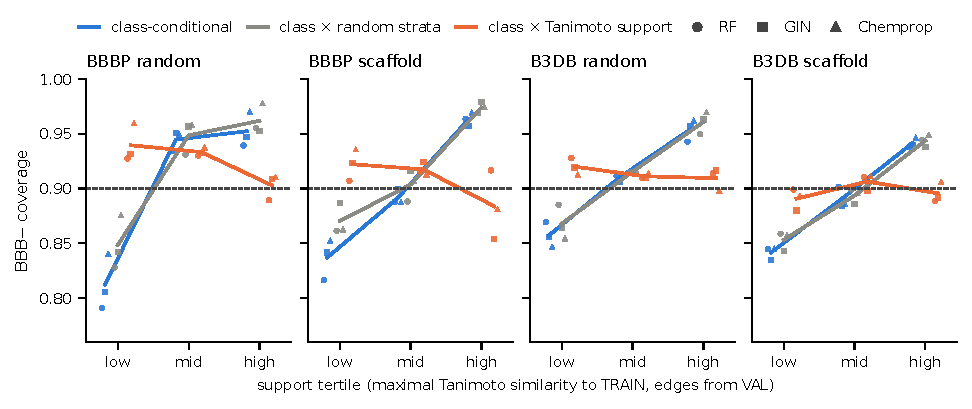
\includegraphics[width=\linewidth]{paper_fig2_hidden_failure_confirmatory.pdf}
\caption{\textbf{Coverage by support tertile.} BBB$-$ coverage under class-conditional calibration, class $\times$ randomly assigned strata of equal size, and class $\times$ Tanimoto support (LAC, $\alpha=0.1$, CE; 20-split means; markers: backbones; lines: their average). Dashed line: target. Intervals: Supplementary Tables~S4 and S9.}\label{fig:hidden}
\end{figure}

\subsection{Why one class threshold fails (RQ2, exploratory)}\label{sec:mechanism}
Class-conditional calibration applies one threshold to every BBB$-$ compound, so the coverage of low- and high-support BBB$-$ compounds differs whenever their score distributions place different probability below that threshold. They do. From the highest to the lowest support tertile, the mean predicted probability of the true class falls by \V{mech.p2.min.min}--\V{mech.p2.min.max} for BBB$-$ compounds and by \V{mech.p2.maj.min}--\V{mech.p2.maj.max} for BBB$+$ compounds, a larger fall for BBB$-$ in \V{mech.p2.n} of 12 cells (Supplementary Table~S13). Familiar BBB$-$ compounds therefore lie well inside the shared threshold and unfamiliar ones beyond it, the situation of Proposition~\ref{prop:shared}. At a fixed predicted probability, lower support also predicts a higher observed BBB$-$ rate on B3DB (support coefficient \V{scal.b3db.coef.min} to \V{scal.b3db.coef.max} per 0.1 Tanimoto, interval below zero in \V{scal.b3db.nneg} of 6 cells): the models under-predict BBB$-$ off-support. On BBBP this calibration effect is inconsistent (\V{scal.bbbp.coef.min} to \V{scal.bbbp.coef.max}). One prediction failed. A purely minority-specific account predicts that low-support BBB$+$ compounds are covered at target; they are covered at \V{mech.covmajlow.min}--\V{mech.covmajlow.max}. Off-support degradation therefore affects both classes; it is asymmetric, not exclusive to BBB$-$. The account is also not sufficient: on Tox21 SR-ARE the minority probability degrades faster as well (\V{mechg.tox21/random.p2min} versus \V{mechg.tox21/random.p2maj}), yet the coverage gap is reversed (Section~\ref{sec:general}). As Proposition~\ref{prop:shared} anticipates, a mean drop is not sufficient: the mass below the shared threshold decides the sign.

\subsection{Joint conditioning repairs the gradient by redistribution (RQ3)}\label{sec:repair}
Class $\times$ support calibration raises low-support BBB$-$ coverage to \V{mx.low.min}--\V{mx.low.max}, while class-level coverage remains \V{mx.cls.min}--\V{mx.cls.max}. The paired gain is \V{gain.min}--\V{gain.max}; it is positive in \V{gain.npos} of 12 cells and significant after Holm correction over the pre-specified family of \V{fam.size} in \V{gain.nsig} (largest significant adjusted $p=\V{gain.sigmaxholm}$). The three cells that do not clear correction are BBBP scaffold for every backbone, with gains of \V{gain.bbbpscaf.min}--\V{gain.bbbpscaf.max} and adjusted $p=\V{gain.bbbpscaf.holm}$; we do not claim a significant repair in that setting. An initial analysis applied Holm correction over the twelve cells of a single backbone, under which these cells were significant; because that was not the pre-specified family, we report the pre-specified one. The cost is \V{size.cost.min}--\V{size.cost.max} labels in mean set size.

\textbf{Targeting, not cell size (exploratory).} Smaller calibration cells can add finite-sample conservativeness whatever the cells are, so part of the gain over class-conditional calibration could come from cell size. Randomly assigned strata of the same number and size isolate this effect: they raise low-support coverage over class-conditional calibration by only \V{rs.cellsize.low.min}--\V{rs.cellsize.low.max}, to \V{rs.randlow.min}--\V{rs.randlow.max}, and raise high-support coverage too (in \V{rs.randhigh.nup} of 12 cells, by up to \V{rs.cellsize.high.max}). That change is comparable to the class-level finite-sample effect bounded in Supplementary Corollary~S1, about $1/(n/3+1)$ (\V{th.csb.bbbp.max} for BBBP, \V{th.csb.b3db.max} for B3DB), although the bound concerns the class rather than the low-support subset. Against this same-cell-size control, class $\times$ Tanimoto cells still raise low-support coverage by \V{rs.gain.min}--\V{rs.gain.max}, positive in \V{rs.npos} of 12 cells and significant after Holm correction over the 12 in \V{rs.nsig} (the exceptions are BBBP scaffold GIN and random forest, adjusted $p\le\V{rs.nonsig.maxholm}$), at a similar set size (\V{rs.mxsize.min}--\V{rs.mxsize.max} versus \V{rs.randsize.min}--\V{rs.randsize.max}; Supplementary Table~S9). Cell-size effects alone therefore do not account for the repair, and the contrast with Mondrian slightly overstates it.

The gain is a redistribution. Joint conditioning lowers high-support BBB$-$ coverage in \V{mx.high.ndrop} of 12 cells, from \V{mond.high.min}--\V{mond.high.max} to \V{mx.high.min}--\V{mx.high.max}: the over-coverage that class-conditional calibration placed on familiar compounds is moved to unfamiliar ones. The high-support point estimate falls below 0.90 in \V{mx.high.nbelow} cells, but its interval lies entirely below 0.90 in \V{mx.high.nciexcl}, consistent with per-cell validity, which is guaranteed only for random splits.

\textbf{Split dependence.} Resampling unique test molecules (\V{boot.nmol.min}--\V{boot.nmol.max} low-support BBB$-$ molecules per setting), each drawn once for every split in which it appears, leaves \V{boot.molecule.nsig} of 12 gains significant after Holm correction (lower 95\% bounds \V{boot.molecule.cilo.min}--\V{boot.molecule.cilo.max}); resampling scaffolds gives \V{boot.scaffold.nsig} of 12. This resampling treats test molecules as the unit while holding the trained models and calibration sets fixed, so it is a sensitivity analysis for molecules recurring across splits, not a replacement for the pre-specified test.

\textbf{Robustness (exploratory).} The gain is positive in \V{sec.aps.npos} of 12 cells for APS, \V{sec.raps.npos} for RAPS, \V{sec.a05.npos} at $\alpha=0.05$ and \V{sec.a20.npos} at $\alpha=0.20$; at $\alpha=0.20$, class-conditional low-support coverage falls to \V{sec.a20.mondlow.min}--\V{sec.a20.mondlow.max} against a target of 0.80. Evaluated on the same tertiles, alternative support definitions give low-support coverage of \V{rob.mondrian_x_maccs.min}--\V{rob.mondrian_x_maccs.max} (MACCS), \V{rob.mondrian_x_top5.min}--\V{rob.mondrian_x_top5.max} (top-5 Tanimoto), \V{rob.mondrian_kmeans3.min}--\V{rob.mondrian_kmeans3.max} ($k$-means) and \V{rob.mondrian_tpsa.min}--\V{rob.mondrian_tpsa.max} (TPSA strata), whereas randomly assigned strata give \V{rob.mondrian_x_random.min}--\V{rob.mondrian_x_random.max} (Supplementary Tables~S7 and S8). Among the alternatives evaluated, similarity-based supports behave like Tanimoto support, whereas $k$-means clusters and TPSA strata land close to random strata. Weighted cross-entropy does not remove the support gradient (Supplementary Table~S11), and temperature scaling and logit adjustment leave class-conditional and class $\times$ support sets unchanged (largest difference \V{inv.la.max} in set size, from ties; Supplementary Proposition~S4).

\subsection{Existing conditional conformal methods (RQ3, exploratory)}\label{sec:existing}
Methods that condition on class or reweight globally leave the gradient: low-support BBB$-$ coverage is \V{cb.rc3p.low.min}--\V{cb.rc3p.low.max} for rank calibration~\cite{shi2024rc3p} (interval below target in \V{cb.rc3p.nfail} of 12 cells), \V{cb.clustered_cells.low.min}--\V{cb.clustered_cells.low.max} for clustered calibration~\cite{ding2023clustered} applied to class $\times$ support cells (\V{cb.clustered_cells.nfail}), \V{cb.interp_q90.low.min}--\V{cb.interp_q90.low.max} for interpolation between marginal and class-conditional calibration~\cite{ding2026longtail} (\V{cb.interp_q90.nfail}), and \V{cb.kmm_mondrian.low.min}--\V{cb.kmm_mondrian.low.max} for kernel-mean-matching weights~\cite{laghuvarapu2026kmmcp} (\V{cb.kmm_mondrian.nfail}). Methods that localize on support repair it: group-conditional quantile regression in the style of Kandinsky conformal prediction~\cite{bairaktari2025kandinsky} (\V{cb.kandinsky_qr.nfail} cells failing, set size \V{cb.kandinsky_qr.size}), conditional calibration on support~\cite{gibbs2025conditional} (\V{cb.condqr_sim.nfail}, \V{cb.condqr_sim.size}), randomly localized conformal prediction~\cite{hore2025rlcp} (\V{cb.rlcp_sim.nfail}, \V{cb.rlcp_sim.size}) and Tanimoto-kernel localized conformal prediction~\cite{guan2023lcp} (\V{cb.lcp_tanimoto.nfail}, \V{cb.lcp_tanimoto.size}), compared with \V{cb.mondrian_x.nfail} and \V{cb.mondrian_x.size} for the fixed partition. A training-conditional Mondrian threshold~\cite{vovk2012conditional} reduces failing cells to \V{cb.mondrian_pac.nfail} by raising coverage everywhere (set size \V{cb.mondrian_pac.size}). Several are our approximations of the published methods (Supplementary Table~S12). Conditioning on support repairs the gradient whatever the construction, and the fixed partition does so at among the smallest set sizes.

\subsection{Calibration sparsity and the limits of adaptive merging (RQ3)}\label{sec:merge}
Joint conditioning divides an already small minority calibration set (\V{cg.ncalmin.min}--\V{cg.ncalmin.max} BBB$-$ molecules per split). Subsampling this set shows that the fraction of class $\times$ support cells too sparse for a finite threshold is about one half when strata receive only a few BBB$-$ calibration molecules and falls steeply as they approach and exceed $\nreq=11$ (Supplementary Fig.~S1). The Beta-law budget, fixed before the confirmatory runs, therefore predicts the measured feasibility threshold and yields a planning heuristic, not a guarantee, $B\le n^{-}_{\mathrm{cal}}/\nreq(\alpha)$: at $\alpha=0.1$, at most five strata for BBBP-sized and about nineteen for B3DB-sized minority calibration sets.


Count-based merging was designed for this regime but does not improve on a fixed partition. All partitions are scored on the same lowest VAL tertile, so that low support denotes the same molecules for every number of strata. At the realized calibration sizes, merging on three strata leaves low-support BBB$-$ coverage unchanged in \V{cg.all.sabm_eq_b3} of \V{cg.ncells.all} cells (largest difference in the primary family \V{sabmfixed.maxabs}); it fires only in BBBP splits where a fixed cell is too sparse for a finite threshold, where it reduces mean set size by up to \V{cg.all.sabm3.size_maxdiff} (identical in \V{cg.all.sabm3.size_eq} of 12 cells). Merging on eight strata trades informativeness for coverage relative to a fixed two-stratum partition, which yields more singleton sets (\V{cgm.all.fixed_b2.singleton_rate} versus \V{cgm.all.sabm_b8.singleton_rate}) and smaller sets (\V{cgm.all.fixed_b2.set_size} versus \V{cgm.all.sabm_b8.set_size}) at slightly lower low-support coverage (\V{cgm.all.fixed_b2.cov_min_t0} versus \V{cgm.all.sabm_b8.cov_min_t0}); the same ordering holds with 40 BBB$-$ calibration molecules (singleton rate \V{cgm.40.fixed_b2.singleton_rate} versus \V{cgm.40.sabm_b8.singleton_rate}). With 20, merging reverts to class-conditional calibration and its low-support coverage (\V{cgm.20.sabm_b8.cov_min_t0}) equals that of Mondrian (\V{cgm.20.mondrian.cov_min_t0}): it preserves informative sets only by relinquishing the conditioning it was introduced to provide, which Theorem~\ref{thm:sabm} permits because its guarantee concerns merged groups. At that size the design rule allows a single stratum, that is, class-conditional calibration, so a coarse fixed partition sized by the rule gives the same answer without merging.

\subsection{Failures shared across architectures and their chemistry (RQ4)}\label{sec:persistent}
If the gradient reflected idiosyncrasies of individual models, different backbones would miss different compounds. On B3DB random, the random forest, GIN and Chemprop are persistently wrong on \V{pf.b3db/random.rf}, \V{pf.b3db/random.gin} and \V{pf.b3db/random.chemprop} of \V{pf.b3db/random.n_eligible} eligible BBB$-$ molecules, and \V{pf.b3db/random.n_cross_arch} are missed by all three at every appearance, against \V{pf.b3db/random.null} expected if backbones failed independently (permutation $p<0.001$); on B3DB scaffold the counts are \V{pf.b3db/scaffold.n_cross_arch} against \V{pf.b3db/scaffold.null}. Backbones share molecules and splits, so some agreement is expected from shared difficulty; permuting within strata of support and TPSA as well raises the expected counts only to \V{cc.b3db/random.nullcov} and \V{cc.b3db/scaffold.nullcov} ($p\le\V{cc.b3db/scaffold.pcov}$). A strict failure is missed at each of its $k\ge2$ test appearances; on B3DB the median $k$ is \V{cc.b3db/random.kmed} and \V{cc.b3db/scaffold.kmed}, and \V{cc.b3db/random.n_kge3} and \V{cc.b3db/scaffold.n_kge3} of these molecules were tested at least three times (Supplementary Table~S15). The strict definition yields \V{pf.bbbp/random.n_cross_arch} molecules on BBBP random, \V{pf.bbbp/scaffold.n_cross_arch} on BBBP scaffold and none under transfer, where a molecule must be missed in all 20 splits. The descriptive majority rule yields \V{pf.bbbp/random.n_majority_all3}, \V{pf.bbbp/scaffold.n_majority_all3}, \V{pf.b3db/random.n_majority_all3}, \V{pf.b3db/scaffold.n_majority_all3} and \V{pf.bbbptob3db/scaffold.n_majority_all3} molecules for the five settings.

\textbf{Label and curation checks.} Of the BBBP molecules, \V{la.overlap}\% also occur in B3DB by connectivity key; labels agree for \V{la.agree}\% of them and differ for \V{la.ndis}, \V{la.negpos} of which are BBB$-$ in BBBP and BBB$+$ in B3DB. On BBBP, persistent failures are enriched for such conflicts (majority rule: odds ratio \V{la.bbbp/random.majority.or}, Fisher $p=\V{la.bbbp/random.majority.p}$, random; \V{la.bbbp/scaffold.majority.or}, $p=\V{la.bbbp/scaffold.majority.p}$, scaffold), and both BBBP cross-architecture failures, thiopental and phenylbutazone, are BBB$+$ in B3DB. A disagreement does not show which label is correct, so these molecules are treated as ambiguous and chemical interpretation rests on B3DB, where no conflicting molecule is a failure. Inspection of the B3DB failures found three curation errors, each verifiable from the records: a BBB$-$ record named rifampin whose structure is an unrelated difluoropyridine amide (record 3838), and BBB$-$ records of phenylbutazone and cyclobenzaprine (records 5692 and 5253, one reference each) drawn so that they escape de-duplication against correctly drawn BBB$+$ records of the same compounds (records 279 and 1009). A name-level screen finds a same-name BBB$+$ record for \V{nc.b3db/random.strict.ratefail}\% and \V{nc.b3db/scaffold.strict.ratefail}\% of strict failures against \V{nc.b3db/random.strict.raterest}\% of other eligible BBB$-$ molecules (Fisher $p=\V{nc.b3db/random.strict.p}$ and \V{nc.b3db/scaffold.strict.p}). Removing the three records from calibration and test leaves \V{pfx.b3db/random.n_cross_arch} and \V{pfx.b3db/scaffold.n_cross_arch} cross-architecture failures on B3DB random and scaffold (Supplementary Section~F).

\textbf{Physicochemistry.} Strictly persistent BBB$-$ failures on B3DB have median TPSA of \V{pd.str.b3db/random.TPSA.med} and \V{pd.str.b3db/scaffold.TPSA.med}\,\AA$^2$ (random and scaffold), compared with \V{pd.str.b3db/random.TPSA.rest} and \V{pd.str.b3db/scaffold.TPSA.rest}\,\AA$^2$ for other eligible BBB$-$ compounds (Fig.~\ref{fig:persistent}). Under the majority rule, which populates all five settings, the TPSA difference holds in every setting (for example \V{pd.maj.bbbp/random.TPSA.med} versus \V{pd.maj.bbbp/random.TPSA.rest}\,\AA$^2$ on BBBP random and \V{pd.maj.bbbptob3db/scaffold.TPSA.med} versus \V{pd.maj.bbbptob3db/scaffold.TPSA.rest}\,\AA$^2$ under transfer; Holm $p\le\V{pd.maj.tpsa.maxholm}$ over \V{pd.maj.ntests} tests), with fewer H-bond donors throughout; molecular weight is lower on B3DB and under transfer, and cLogP differs significantly only on BBBP random. These compounds are labelled non-permeant but have physicochemistry typical of CNS-penetrant drugs~\cite{wager2010cnsmpo}; some may be genuine exceptions, for example through efflux, others noisy labels. Across all BBB$-$ test appearances, the association between low TPSA and being missed persists after adjustment for chemical support in \V{adj.nsup} of \V{adj.ncells} backbone $\times$ setting cells, and permuting TPSA within support tertiles never reproduces it; with molecular weight and cLogP also included it remains significant in \V{adj.nfull} of \V{adj.ncells}, the exception being BBBP scaffold for every backbone (Supplementary Table~S18). We therefore report a reproducible physicochemical association that is largely distinct from chemical support, and we do not infer a transport mechanism. Rule-selected examples with their nearest never-missed controls are shown in Supplementary Fig.~S9.

\begin{figure}[t]
\centering
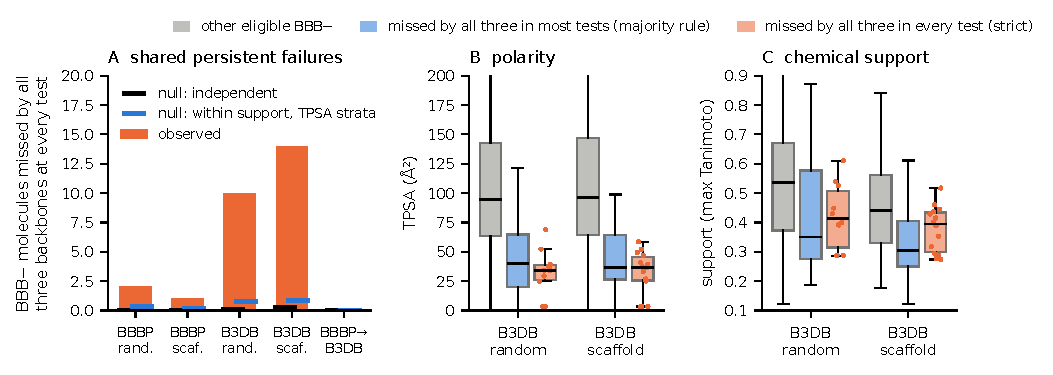
\includegraphics[width=\linewidth]{paper_fig3_persistent_failures_ce.pdf}
\caption{\textbf{Failures shared across architectures.} (A) BBB$-$ molecules missed by all three backbones at every test appearance, against two permutation nulls: independent failures within strata of the number of appearances (black) and, in addition, within support and TPSA tertiles (blue). (B, C) TPSA and support of strict and majority-rule failures and of other eligible BBB$-$ molecules on B3DB (boxes: quartiles; points: strict failures). Unique molecules, seeds 100--119; association only. Structures and dataset flags: Supplementary Fig.~S7.}\label{fig:persistent}
\end{figure}

\subsection{Screening decisions (RQ5)}\label{sec:screening}
Interpreted as triage decisions (a singleton is accepted, any other set deferred), support conditioning changes little relative to class-conditional calibration alone: the fraction of BBB$-$ compounds accepted as BBB$+$ changes by \V{su.mondrian.minority_false_accept_rate.exch.min} to \V{su.mondrian.minority_false_accept_rate.exch.max} on the in-domain settings and \V{su.mondrian.minority_false_accept_rate.tr.min} to \V{su.mondrian.minority_false_accept_rate.tr.max} under transfer, at \V{su.mondrian.deferral_rate.exch.min} to \V{su.mondrian.deferral_rate.exch.max} more deferral (Fig.~\ref{fig:screen}). The strongest baseline therefore adds a rejection filter to class-conditional calibration and defers, among its accepted calls, the compounds with the lowest support or confidence until deferral matches that of class $\times$ support. Against class-conditional calibration with an applicability-domain filter, the change is \V{cr.mond_ad.minority_false_accept_rate.exch.min} to \V{cr.mond_ad.minority_false_accept_rate.exch.max} (interval excluding zero in \V{cr.mond_ad.minority_false_accept_rate.nlow} of 15 cells), and with thresholds set on VAL \V{cr.mond_ad_val.minority_false_accept_rate.exch.min} to \V{cr.mond_ad_val.minority_false_accept_rate.exch.max}: at the same deferral we find no difference between the two policies on this decision (no equivalence margin was pre-specified). With a confidence filter instead, class $\times$ support accepts fewer BBB$-$ compounds as BBB$+$ (\V{cr.mond_conf.minority_false_accept_rate.exch.min} to \V{cr.mond_conf.minority_false_accept_rate.exch.max}; \V{cr.mond_conf.minority_false_accept_rate.nlow} of 15 cells) at a higher error among accepted calls, and the gains over rejection rules without conformal calibration are larger (applicability domain \V{su.ad_reject.minority_false_accept_rate.exch.min} to \V{su.ad_reject.minority_false_accept_rate.exch.max}; confidence \V{su.conf_reject.minority_false_accept_rate.exch.min} to \V{su.conf_reject.minority_false_accept_rate.exch.max}; Supplementary Tables~S19 and S20). For triage, the value lies in deferring unfamiliar compounds, which a support filter on class-conditional calibration also achieves.

\begin{figure}[t]
\centering
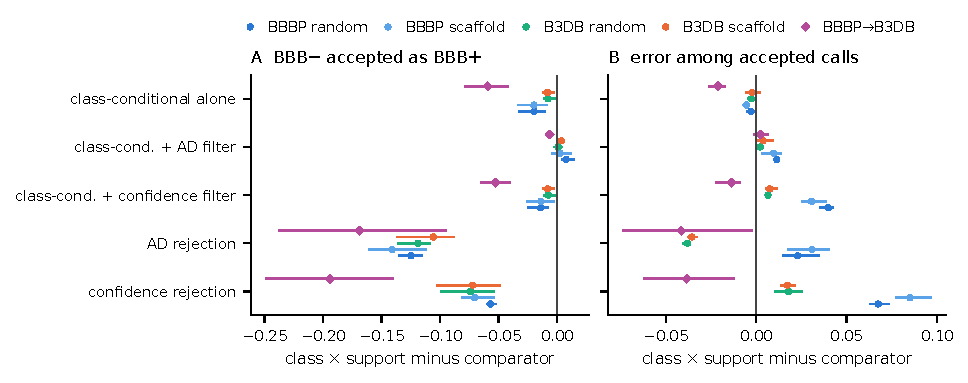
\includegraphics[width=\linewidth]{paper_fig4_screening_utility.pdf}
\caption{\textbf{Screening decisions at $\alpha=0.1$}, class $\times$ support minus each comparator (negative in A favours class $\times$ support). Filters and rejection rules are matched on each split to the deferral of class $\times$ support without test labels. Points: mean over backbones of the 20-split means; bars: range over backbones.}\label{fig:screen}
\end{figure}

\subsection{Shift, other tasks and the prior protocol (RQ6, exploratory)}\label{sec:general}\label{sec:shift}
Under BBBP$\to$B3DB transfer and cluster holdout, where Assumption~\ref{ass:E} is not guaranteed, class $\times$ support moves the random forest's low-support BBB$-$ coverage from \V{e.bbbptob3db/scaffold.rf.mondrian.cov_min_bin0} to \V{e.bbbptob3db/scaffold.rf.mondrian_x.cov_min_bin0} (transfer), \V{e.bbbp/cluster.rf.mondrian.cov_min_bin0} to \V{e.bbbp/cluster.rf.mondrian_x.cov_min_bin0} (BBBP cluster) and \V{e.b3db/cluster.rf.mondrian.cov_min_bin0} to \V{e.b3db/cluster.rf.mondrian_x.cov_min_bin0} (B3DB cluster; empirical, Supplementary Table~S6). Under the BBBP protocol of the closest prior work~\cite{tursunbadalov2026quiet} on seeds 100--119, class-conditional calibration again leaves low-support minority compounds below target (random forest \V{tc.rf.mondrian.low}, graph convolutional network \V{tc.gcn.mondrian.low}, against \V{tc.rf.mondrian.high} and \V{tc.gcn.mondrian.high} at high support), and class $\times$ support raises them by \V{tc.rf.gain} and \V{tc.gcn.gain} (Holm $p=\V{tc.rf.holm}$ and \V{tc.gcn.holm}). On BACE, the same masking and repair appear (random: low \V{gen.bace/random.mondrian.low}, high \V{gen.bace/random.mondrian.high}, gain \V{gen.bace/random.gain}, Holm $p=\V{gen.bace/random.holm}$ over six cells; scaffold: gain \V{gen.bace/scaffold.gain}, $p=\V{gen.bace/scaffold.holm}$). On Tox21 SR-ARE the gap is reversed: low-support actives are covered at \V{gen.tox21/random.mondrian.low} and \V{gen.tox21/scaffold.mondrian.low} and high-support actives at \V{gen.tox21/random.mondrian.high} and \V{gen.tox21/scaffold.mondrian.high}, and support conditioning does not help (gains \V{gen.tox21/random.gain} and \V{gen.tox21/scaffold.gain}). ClinTox, with \V{gen.clintox/random.ncalmin} minority calibration molecules per split, is too sparse to evaluate. The masking is therefore neither specific to BBB nor universal (Supplementary Table~S14): where coverage concentrates depends on the task, which is why it must be measured.

% ------------------------------------------------------------------ 7 DISCUSSION
\section{Discussion and conclusion}\label{sec:discussion}\label{sec:conclusion}
Class-level validity does not imply reliability across chemical space. Class-conditional calibration is the appropriate first step for imbalanced BBB screening, but its guarantee leaves coverage within a class unconstrained, and here coverage concentrates on familiar compounds. The impossibility of informative distribution-free conditional coverage~\cite{barber2021limits} says that some subgroup can fail; here the failing subgroup is identified by a quantity computed before any assay, the direction is accounted for by an asymmetric loss of confidence in the true class off-support, and Proposition~\ref{prop:floor} bounds the size of the failure. Tox21 SR-ARE shows where this account stops. The repair is a standard taxonomy refinement whose effect survives a same-cell-size control and is reproduced by support-aware conformal methods but not by class-level ones. For triage decisions, an applicability-domain filter added to class-conditional calibration achieves a similar benefit, so the case for support conditioning rests on stratum-level coverage. Several shared failures are curation errors or dataset disagreements, which per-molecule analysis exposes. We claim no new method; the contribution is a characterization, with explanation, controls and limits, of how the accepted remedy behaves across chemical support, and the recommendation that, because the pattern is task-dependent, molecular conformal studies report coverage by applicability-domain support with the number of minority calibration compounds per stratum.

\textbf{Limitations.}\label{sec:limits} Finite-sample guarantees hold for random splits only; scaffold, cluster and transfer coverage is empirical. The twenty splits quantify sensitivity to the partition of fixed datasets, not uncertainty over new datasets. BBBP scaffold is the weakest setting, with three of twelve primary cells not significant. Both benchmarks contain label noise and curation errors, some of which we identify. The transfer set is overlap-controlled by connectivity key, which does not establish independent assay provenance. The descriptor association cannot be separated from size, lipophilicity and support on BBBP scaffold, and active efflux could not be examined because the public P-glycoprotein data available to us measure inhibition rather than substrate status. The mechanism analysis is associational and does not identify why models lose confidence off-support. Analyses beyond the primary family were specified afterwards, and several baselines approximate the published algorithms. Persistent failures rest on two to six test appearances per molecule. Calibration-set diagnostics are too noisy to flag a failure in a single deployment (Spearman \V{ca.rho} between leave-one-out calibration and test coverage), although they agree with test outcomes in \V{ca.cellagree} of 12 settings.

\textbf{Code and data availability.} Code, curated data, splits, cached predictions and one command per table and figure: \url{https://github.com/sanjeda-sara/conformal-chemical-support/}. B3DB is distributed under CC0 and BBBP through MoleculeNet.

\bibliographystyle{abbrvnat}
{\small\bibliography{references_final}}
\end{document}